\section{Introduction}
\label{motivation_engagement_introduction}
In this chapter we will discuss the concept of motivation and how it can be used to describe the interactions that individuals have with particular objects or activities. 

We will first provide a general introduction to the construct of motivation followed by a short historical review of theories of reward-driven motivation. We will then focus on how these led to the incentive salience hypothesis formulated by Berridge and Robinson \cite{berridge1998role}. While acknowledging the contribution of other theories in the definition of motivation (and reward-driven motivation in particular) this thesis will mostly focus on the areas of behavioural and affective neuroscience and make use of the framework provided by Berridge and Robinson \cite{berridge1998role}. The reason behind this choice lies in the fact that we found incentive salience to be more specific to motivation and most importantly to have a more robust and clear connection to behaviour. The chapter will then provide a description of the concept of engagement highlighting and how this can be seen as a behavioural derivation of the latent states generated by motivational processes. We will contextualise engagement in the context of videogames presenting a quick overview of the various taxonomies describing how different videogames structural characteristics fuel the motivational processes underlying the engagement behaviour. The chapter closes presenting various approaches for measuring, describing and predicting both engagement and motivation, with a particular focus on the challenges derived by their application in situations where large-scale behavioral telemetry data about user behavior are available.

\section{Motivation as a Reward-Driven Process}
\label{motivation}
The construct of motivation is a key concept for understanding why individuals seek out specific objects or experiences at particular times and why they react in particular ways when encountering objects considered of particular relevance \cite{berridge2004motivation}. In this view motivation can be defined as the process leading to the modulation and reiteration of goal directed behaviours that once reached exerts positive effects on the individual \cite{simpson2016behavioral}. A formal definition of motivation should encompass both the behavioural and the underlying psychobiological level. We will focus first on behavioural aspects of the process and outline in the following sections a theoretical account of motivation which also covers the psychobiological level. 

As we mentioned before, motivation describes why individuals react in particular ways when encountering objects regarded of high relevance and why they approach those objects at particular times \cite{berridge2004motivation}. These type of objects are said to possess "rewarding properties", which can be defined as the positive value ascribed to an object, a behavioral act or an internal physical state as the result of an active process of the mind and the brain \cite{schultz1997neural,berridge2008affective}. Importantly, motivation is not just driven by the fulfilment of fundamental needs like nutrition or reproduction (so-called "primary reward objects" \cite{schultz2000reward}) or the avoidance of negative consequences like physical pain. It also extends to those volitional objects and activities which do not appear to be necessary for the survival of the individual (i.e., "secondary reward objects" \cite{berridge2008affective,sescousse2013processing}). For those activities the expectation of the amount of reward received is learned over time and may vary significantly between individuals \cite{berridge2008affective,simpson2016behavioral}. In spite of this, it would be inefficient to have dedicated and specialized motivational systems for every combination of individuals and objects (e.g., an individual's motivation for playing sport or eating food). Instead, we can think of motivation as a single overarching entity that controls the interaction between individuals and objects in an agnostic manner \cite{simpson2016behavioral}. An analogy may be drawn with the geometric concept of a vector. Looking at Figure \ref{fig: vect_mot} we can imagine the focus on a specific object being represented by the angle of the vector while its length is the intensity of the motivational process (or the amount of motivated behaviour) \cite{simpson2016behavioral}. This, can be thought as a dynamic quantity defined by the state of the individual and the rewarding properties of the object \cite{toates1994comparing,berridge2004motivation,zhang2009neural}.
\begin{figure}[h]
  \begin{center}
    \begin{adjustbox}{width=0.5\columnwidth}
        \tikzset{every picture/.style={line width=0.75pt}} %set default line width to 0.75pt        
            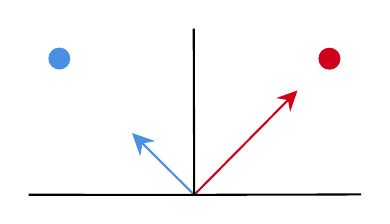
\begin{tikzpicture}[x=0.75pt,y=0.75pt,yscale=-1,xscale=1]
            %uncomment if require: \path (0,300); %set diagram left start at 0, and has height of 300
            
            %Straight Lines [id:da17586827840068286] 
            \draw [color={rgb, 255:red, 208; green, 2; blue, 27 }  ,draw opacity=1 ]   (190.24,200.32) -- (237.89,152.16) ;
            \draw [shift={(240,150.03)}, rotate = 494.69] [fill={rgb, 255:red, 208; green, 2; blue, 27 }  ,fill opacity=1 ][line width=0.08]  [draw opacity=0] (9.82,-4.72) -- (0,0) -- (9.82,4.72) -- (6.52,0) -- cycle    ;
            %Straight Lines [id:da23704064540856618] 
            \draw [color={rgb, 255:red, 74; green, 144; blue, 226 }  ,draw opacity=1 ]   (190.24,200.32) -- (162.38,172.64) ;
            \draw [shift={(160.25,170.53)}, rotate = 404.81] [fill={rgb, 255:red, 74; green, 144; blue, 226 }  ,fill opacity=1 ][line width=0.08]  [draw opacity=0] (10.72,-5.15) -- (0,0) -- (10.72,5.15) -- (7.12,0) -- cycle    ;
            %Shape: Circle [id:dp3839733612485111] 
            \draw  [color={rgb, 255:red, 208; green, 2; blue, 27 }  ,draw opacity=1 ][fill={rgb, 255:red, 208; green, 2; blue, 27 }  ,fill opacity=1 ] (250.58,134.73) .. controls (250.58,132.08) and (252.73,129.93) .. (255.38,129.93) .. controls (258.03,129.93) and (260.18,132.08) .. (260.18,134.73) .. controls (260.18,137.38) and (258.03,139.53) .. (255.38,139.53) .. controls (252.73,139.53) and (250.58,137.38) .. (250.58,134.73) -- cycle ;
            %Shape: Circle [id:dp009447430116501954] 
            \draw  [color={rgb, 255:red, 74; green, 144; blue, 226 }  ,draw opacity=1 ][fill={rgb, 255:red, 74; green, 144; blue, 226 }  ,fill opacity=1 ] (120.47,134.66) .. controls (120.47,132.02) and (122.61,129.88) .. (125.25,129.88) .. controls (127.89,129.88) and (130.03,132.02) .. (130.03,134.66) .. controls (130.03,137.29) and (127.89,139.43) .. (125.25,139.43) .. controls (122.61,139.43) and (120.47,137.29) .. (120.47,134.66) -- cycle ;
            %Straight Lines [id:da5714219654763008] 
            \draw    (190,120.28) -- (190.24,200.32) ;
            %Straight Lines [id:da22247567054966455] 
            \draw    (110.5,200.28) -- (190.24,200.32) ;
            %Straight Lines [id:da4124676757039665] 
            \draw    (270.64,200.12) -- (190.24,200.32) ;
            
            
            
            
            \end{tikzpicture}
    \end{adjustbox}
  \end{center}
\caption{\textbf{Motivation as a vector}. Blue and red dots represent two objects with different characteristics while the two arrows illustrate the hypothetical motivational propensity of an individual (or two individuals) towards them. The black segments delineate the space created by the combination of the objects' characteristics and the motivational propensity of the individuals. Here the red object has the potential to generate more behaviour than the blue object possibly as a result of its characteristics and those of the individual interacting with it.}
\label{fig: vect_mot}
\end{figure}
Summarizing we can say that from a motivational point of view, the behaviour of an individual is driven by the expectancy of pleasurable outcomes derived by the goal the behaviour is aiming to reach \cite{berridge2004motivation}. Therefore, if motivation acts as a single overarching process, we expect it to hold predictive and explanatory power over goal directed behaviour seamlessly across a heterogeneous range of situations and individuals. Motivational theories based on the concepts of reward and incentive are promising candidates for this because, relying on consistent and plausible psychobiological bases, they tend to operate abstracting from the nature of the individuals and the objects. \cite{ikemoto1999role,berridge1998role,salamone2002motivational,berridge2004motivation,armony2013cambridge,corbit2015learning}.

\subsection{An Historical View on Reward-driven Motivation}
\label{motivation_hist}
Introducing the processes of classical and operant conditioning is an essential step for describing theories of reward-driven motivation, in particular if we are interested in their behavioural correlates. Both constructs heavily rely on the general concepts of reinforcer and reinforcement process. Simply put, reinforcers are those objects or actions that have the ability to alter the likelyhood of appearance of specific behaviours \cite{kling1971woodworth,skinner1953science,squire2012fundamental}. A reinforcement process instead define the learning mechanisms by which a specific behaviour becomes, over time, more or less probable conditional on the presence of particular reinforcers \cite{kling1971woodworth}. In this view we can think of classical and operant conditioning as two complementary oprationalizations of the reinforcement process. 
Classical conditioning describes the learning process in which, independently from the activity of an individual, the repeated pairing of two objects will cause one to acquire the eliciting properties of the other \cite{squire2012fundamental}. In other words, the repeated pairing of a neutral object with reinforcing consequences will imbue the first with reinforcement properties making it a reinforcer. 
Operant conditioning on the other hand, extends the concept of classical conditioning introducing the agency of the individual \cite{skinner1953science}. The frequency of behaviour produced by an individual tends to increase when precise consequences are associated to it \cite{skinner1953science}. In this view, an operant is formalized as a goal directed behaviour while all the elements reinforcing the re-iteration of this behaviour are called reinforcers \cite{skinner1953science}. The learning process here results from the relationship between a behaviour and its consequences, therefore the probability of behaviour to take place is related to its capability to generate reinforcer \cite{kling1971woodworth}. 
Both classical and operant conditioning are of course very simplistic accounts of human behaviour, but nevertheless able to succinctly illustrate a fundamental process by which most (if not all) individuals are able to learn and leverage the association between actions and the positive (i.e. rewarding) consequences associated to them. In this regard, it is not surprising that many theories of reward-driven motivation stem directly from these two constructs. 

For example, in his work Bolles \cite{bolles1972reinforcement} suggested that individuals were motivated by the "expectations of incentive outcomes". These expectations are formed through a learning process where an association between actions and potential pleasurable outcomes is created \cite{bolles1972reinforcement,berridge2004motivation}. Expanding on this idea, Bindra \cite{bindra1978adaptive} suggested that the learning process does not just generate pleasure expectations in response to specific behaviours but it also allows individuals to perceive the behaviours themselves as a source of hedonic reward \cite{bindra1978adaptive,berridge2004motivation}.
This introduces the concept of learning through reinforcement: an object and the behaviours associated to it become relevant and salient for an individual as a consequence of learning its incentive properties \cite{berridge2004motivation}. A third theoretical formulation by Toates \cite{toates1994comparing}, asserted that the magnitude of the perceived incentives introduced by both Bolles and Bindra is modulated by the internal states of the individual \cite{toates1994comparing,berridge2004motivation}. In other words, the incentive expectations (and consequently the associated motivated behaviours) learned by an individual can change over time depending on the individual's internal state. 

Until now we have mainly used the terms reinforces and incentives for identifying objects able to drive and shape behaviour, but when it comes to define effective reinforces, it is not just a matter of merely pairing a behaviour with a stimulus but the stimulus itself has to have particular properties. In this view, stimuli able to generate pleasurable feelings in the individual are the best candidates for being effective reinforces, they are said having ‘rewarding properties’. But what is, and how can be defined the reward? The reward is a process generated in response to a stimulus making it desirable for its capacity to generate pleasurable responses. In this view, for being able to generate rewarding response, a stimulus needs two fundamental properties: it has to be wanted (i.e., it acquires the capacity to become desirable) and liked (i.e., it has to be able to generate pleasure in the individual) \cite{berridge2009dissecting}. But how a particular object acquires these properties? This is mostly carried out by the same learning processes mentioned in section \ref{motivation_hist}. The repeated pairing of a stimulus with the (positive) consequences it exerts on the individual will imbue the first with so called rewarding properties. Moreover, through operant conditioning not just the stimulus itself but also the connected instrumental behaviour will likely acquire the same rewarding properties \cite{berridge2009dissecting}. As anticipated in section \ref{motivation}, a useful distinction that can be made is between objects having primary and secondary reward properties. Objects linked with essential evolutionary needs (i.e., satisfaction of homeostatic needs) are on a fast track for becoming reinforcers, their rewarding properties do not have to be learned but are, up to a certain extent, intrinsic to them \cite{sescousse2013processing}. Classical examples of primary rewards are food, mating-related activities and drug abuse \cite{berridge2004motivation, simpson2016behavioral}. On the other hand, objects with so called secondary rewarding properties do not hold an innate capacity to generate pleasurable experiences, this capacity is acquired by means of the same learning mechanisms we have just presented \cite{sescousse2013processing}. 

\subsection{The Incentive Salience Theory of Motivation}
\label{incentive_salience}
The approaches proposed by Bolles, Bindra and Toates,  provide an account of reward-based motivation but they assume that there is no distinction between the affective dimension of an incentive (i.e., how pleasurable it is) and the purely motivational aspect of it (i.e., how much goal directed behaviour it can produce) \cite{bindra1978adaptive,toates1994comparing}. Expanding on this, Berridge and Robinson proposed that the motivational process controlling the interaction between individuals and objects might not be a unitary mechanism but rather a composite process having specific and dissociable components which rely on specialized neurobiological mechanisms, namely: \emph{liking}, \emph{wanting} and \emph{learning} \cite{berridge1998role,berridge2009dissecting,smith2011disentangling}.

\paragraph*{Liking}
\label{liking}
The \emph{liking} component describes the pleasure expected by an individual when interacting with an object \cite{berridge2009dissecting}. It is responsible for the hedonic quality of an experience and acts as a signal indicating that interacting again with that object might be beneficial. Despite the fact that \emph{liking} plays an important role in the incentive salience hypothesis of motivation it is difficult to measure it outside controlled laboratory environments \cite{berridge1998role} and it will not form a central theme of this thesis. Instead, we will focus on the "wanting" and "learning" components.

\paragraph*{Wanting}
\label{wanting}
The \emph{wanting} component, or "incentive salience", has the function of generating and holding latent representation of objects and behavioural acts and of attributing value to them through learning mechanisms. These "valued representations" can then be used by action selection systems in order to make certain behaviours more likely \cite{ikemoto1996dissociations,berridge1998role,mcclure2003computational,berridge2004motivation}. As a consequence of this, when an object is attributed with incentive salience it will more likely draw the subject's attention and become the focus of goal directed behaviours \cite{berridge2004motivation}. Interestingly, \emph{wanting} seems to be more than a simple form of value-caching but rather a dynamic process in constant change \cite{robinson1993neural,zhang2009neural,tindell2009dynamic,berridge2012prediction}. This is because the saliency of an object depends both on its attributed value but also on the state of the individual interacting with it. A change in the individual's internal state can dampen, magnify or even revert the amount of attributed salience. \cite{robinson1993neural,zhang2009neural,tindell2009dynamic,berridge2012prediction}. It is important to note that \emph{wanting} is not the hedonic expectation associated to an object, (which is designated by \emph{liking}), but rather the process promoting the approach towards an object and the interaction with it \cite{berridge2009dissecting,robinson2015roles}. Despite the fact that \emph{liking} and \emph{wanting} are often correlated (i.e. I want what I like and vice versa) they can occasionally be triggered separately: addictive behaviours for instance are a notable example of \emph{wanting} without \emph{liking} \cite{robinson1993neural}. The functional dissociation between these two components is linked to differences in the underlying neurobiological substrate \cite{berridge2009dissecting,smith2011disentangling}. Neurotransmitters and brain areas responsible for \emph{wanting} appear to be more numerous, diverse and easily activated than those for \emph{liking} \cite{berridge2009dissecting,robinson2015roles}. As a consequence, increased incentive salience can be obtained by raising dopamine levels in many portion of the striatum without the need for the synchronized activity in other areas \cite{berridge2009dissecting,smith2011disentangling,meyer2015motivational}. This implies that the \emph{wanting} component tends to produce more robust behavioural indicators in the form of increased amount and frequency of interactions between an individual and an object \cite{berridge1998role}, which makes it a promising candidate for behavioural studies in conditions where strict experimental control is not possible.

\paragraph*{Learning}
\label{learning}
The last component in the formulation proposed by Berridge and Robinson \cite{berridge1998role,berridge2004motivation} consists of mechanisms that provide an individual with the capability to predict, based on past experiences, the occurrence of future pleasurable outcomes (i.e., \emph{liking} reactions) when interacting with specific objects. These are similar to the learning processes illustrated in section \ref{motivation_hist} and have a twofold function. These mechanisms allow the attribution and change of incentive salience properties to previously \emph{liked} objects (e.g., primary reward objects) but they also enable subjects to learn the hedonic value of initially neutral stimuli (e.g., secondary reward objects). The \emph{learning} mechanism is based on classical conditioning: through repeated interactions with an object an individual will learn its hedonic properties and consequently attribute incentive salience to it \cite{berridge2004motivation,berridge2009dissecting}. This process is driven by mechanisms similar to those of reward-prediction error: learning is driven by spikes in dopaminergic activity generated by a mismatch between expected and experienced rewards. \cite{schultz1997neural,schultz2000multiple,flagel2011selective}.

\section{Engagement as a Derivative of Motivation}
\label{engagement}
We will now momentarily diverge from our discussion on motivation in order to introduce the construct of engagement. The reason for this brief detour lies in the fact that presenting the construct of engagement allows us to better understand the practical implication that motivational processes have in our everyday life - and in particular in the context of videogames. Despite engagement has applications in a wide range of contexts, we think it is better understood when framed within a specific class of activities (the reason for this will emerge in the following sections). In this view, given the background from which this work has arisen, we will focus on the area of videogames but we will make evident how, by framing engagement as a byproduct of motivational processes, we can easily generalize it to other type of activities.

\subsection{Theories of Engagement}
\label{factors_engagement}
Playing games has always been present in human history as an occupation aiming to entertain and relax \cite{connolly2012systematic}, it can be defined as a free-time activity with spatial and temporal boundaries able to intensely absorb who is involved in it \cite{connolly2012systematic}. 

A special case of the broader group of games are those delivered and experienced in a digital format (i.e., videogames) which in the last decades has been substituting more traditional playful activities \cite{boyle2012engagement,connolly2012systematic}. This phenomenon has been reflected both in terms of number of people involved in playing videogames as well as in the amount of time spent engaging in this activity \cite{boyle2012engagement, zendle2022transnational}. One of the main reasons for this explosive phenomenon is the fact that videogames seems to be perfect medium for delivering pleasurable experiences \cite{boyle2012engagement}, consequently holding a strong potential to engage and retain users involved in the playing activity. 

Various attempt has been made to understand engagement in videogames, both as unitary process and at the level of factors driving and influencing it, across individuals, communities and societies \cite{boyle2012engagement}. The literature on the subject is abundant although extremely heterogeneous \cite{boyle2012engagement}, with no clear consensus even around key terms and definitions. A clear example of this heterogeneity is the definition of engagement provided by O'Brien et al. \cite{o2008user}:

\textit{"...a quality of user experiences with technology that is characterized by challenge, aesthetic and sensory appeal, feedback, novelty, interactivity, perceived control and time, awareness, motivation, interest and affect..."}

this definition, although providing a good holistic description, makes it exceptionally hard to clearly define a unitary framework for defining and measuring engagement let alone specifying its mechanistic aspects. This lack of theoretical formalism is reflected in most (if not all) accounts of engagement and, to a certain extent, inevitable given the breadth of the behavioural, cognitive and affective aspects that the construct tries to cover. This can in part be understood and justified by the strong inter-disciplinarity characterising the research on videogames engagement. Indeed it is not uncommon to find contribution to the subject within humanities, natural and technical sciences, management, business and more, which each field relying on with their own terminologies and weltanschauungs. Nevertheless, inspecting some of the most prominent theories associated to the concept of engagement, we can individuate some common themes useful for composing a unified framework.

\paragraph*{Flow} This is a classical construct often occurring in the videogame literature for explaining the phenomenon of engagement. Developed by Csikszentmihalyi \cite{csikszentmihalyi2014toward}, the construct of flow prescribes that when an individual is absorbed in an activity perceived as valuable they will experience a rewarding state of optimal pleasure constituting the fuel for the engagement process \cite{boyle2012engagement}. In this view, conditio sine qua non for the flow state to arise is a balanced combination of the individual’ state level and the characteristics of the interaction in which they are involved \cite{boyle2012engagement,csikszentmihalyi2014toward}. Despite offering an interesting point of view, the concept of flow as a framework for explaining engagement might be prone to the fallacy of circular reasoning: is an individual engaged in a specific activity because this provides the optimal flow experience or this last one is a bi-product of being engaged in the activity itself? 

\paragraph*{Immersion} This construct is closely connected to that of flow but specifically concerned with the psychological experience of engaging with a computer game \cite{jennett2008measuring}. Immersion tries to describe the experience of engaging in a specific moment in time with a videogame  rather than posing itself as a factor influencing or driving engagement \cite{jennett2008measuring}. According to Jennet et al. \cite{jennett2008measuring}, as a result of a good gaming experience, an individual might loose track of time and space and will experience a sense of being completely "immersed" in the playing activity.

\paragraph*{Uses and gratification} This theory states that the consumption of media is a way for individuals to satisfy the need for gratification (i.e., reward). The gratification-seeking behaviour is then driven and characterized by the nature of the underlying motive generating them (e.g., my need to connect with other people drives my social-media consumption) \cite{lucas2004sex}. Again, according to this theory, individuals are not passive bystanders but will actively interact with a specific media object based on its ability to meet the individual's underlying motivational drive. Uses and gratification theory introduce two important concepts: first that individuals engage in a spontaneous activity (i.e., media object interaction) in search of some form of gratification and second that this interaction is not passive but rather an active process.

\subsubsection{The Engagement Process Model}
\label{eng_proc_model}
We will focus now on a relatively atypical formalization of the construct of engagement, the engagement process model formulated by O'Brien and colleagues \cite{o2008user}. 

This framework, instead of presenting engagement as a static entity proposes the idea that it is better understood as a dynamic process \cite{o2008user}. O'Brien et al. avoid to give an exact definition of engagement but rather describe it as a process with distinct phases each one possessing peculiar attributes \cite{o2008user}:
\begin{figure}[h]
\begin{center}
\begin{adjustbox}{width=\textwidth}

% Gradient Info
  
\tikzset {_2yn49zl61/.code = {\pgfsetadditionalshadetransform{ \pgftransformshift{\pgfpoint{0 bp } { 0 bp }  }  \pgftransformrotate{0 }  \pgftransformscale{2 }  }}}
\pgfdeclarehorizontalshading{_f0h1xn2np}{150bp}{rgb(0bp)=(0.88,0.88,0.88);
rgb(37.5bp)=(0.88,0.88,0.88);
rgb(49.53571319580078bp)=(0.88,0.88,0.88);
rgb(62.5bp)=(1,0,0);
rgb(100bp)=(1,0,0)}
\tikzset{_ao557rzfs/.code = {\pgfsetadditionalshadetransform{\pgftransformshift{\pgfpoint{0 bp } { 0 bp }  }  \pgftransformrotate{0 }  \pgftransformscale{2 } }}}
\pgfdeclarehorizontalshading{_b1qqyoil7} {150bp} {color(0bp)=(transparent!61);
color(37.5bp)=(transparent!61);
color(49.53571319580078bp)=(transparent!75);
color(62.5bp)=(transparent!75);
color(100bp)=(transparent!75) } 
\pgfdeclarefading{_gj5ns3oqm}{\tikz \fill[shading=_b1qqyoil7,_ao557rzfs] (0,0) rectangle (50bp,50bp); } 

% Gradient Info
  
\tikzset {_5ocf120kv/.code = {\pgfsetadditionalshadetransform{ \pgftransformshift{\pgfpoint{0 bp } { 0 bp }  }  \pgftransformrotate{0 }  \pgftransformscale{2 }  }}}
\pgfdeclarehorizontalshading{_25n4qjk0b}{150bp}{rgb(0bp)=(1,0,0);
rgb(37.5bp)=(1,0,0);
rgb(62.5bp)=(0,0,1);
rgb(100bp)=(0,0,1)}
\tikzset{_m8uedxkdp/.code = {\pgfsetadditionalshadetransform{\pgftransformshift{\pgfpoint{0 bp } { 0 bp }  }  \pgftransformrotate{0 }  \pgftransformscale{2 } }}}
\pgfdeclarehorizontalshading{_49t70h8cn} {150bp} {color(0bp)=(transparent!75);
color(37.5bp)=(transparent!75);
color(62.5bp)=(transparent!75);
color(100bp)=(transparent!75) } 
\pgfdeclarefading{_ugfmlo9rg}{\tikz \fill[shading=_49t70h8cn,_m8uedxkdp] (0,0) rectangle (50bp,50bp); } 

% Gradient Info
  
\tikzset {_daocnbh0q/.code = {\pgfsetadditionalshadetransform{ \pgftransformshift{\pgfpoint{0 bp } { 0 bp }  }  \pgftransformrotate{0 }  \pgftransformscale{2 }  }}}
\pgfdeclarehorizontalshading{_03e54ezl1}{150bp}{rgb(0bp)=(0,0,1);
rgb(37.5bp)=(0,0,1);
rgb(62.5bp)=(0,0,1);
rgb(100bp)=(0,0,1)}
\tikzset{_48is8yhe5/.code = {\pgfsetadditionalshadetransform{\pgftransformshift{\pgfpoint{0 bp } { 0 bp }  }  \pgftransformrotate{0 }  \pgftransformscale{2 } }}}
\pgfdeclarehorizontalshading{_w9dk1nw55} {150bp} {color(0bp)=(transparent!75);
color(37.5bp)=(transparent!75);
color(62.5bp)=(transparent!50);
color(100bp)=(transparent!50) } 
\pgfdeclarefading{_thlshpcj1}{\tikz \fill[shading=_w9dk1nw55,_48is8yhe5] (0,0) rectangle (50bp,50bp); } 

% Gradient Info
  
\tikzset {_2e7ef02nx/.code = {\pgfsetadditionalshadetransform{ \pgftransformshift{\pgfpoint{0 bp } { 0 bp }  }  \pgftransformrotate{0 }  \pgftransformscale{2 }  }}}
\pgfdeclarehorizontalshading{_qf8n4pbxh}{150bp}{rgb(0bp)=(1,0,0);
rgb(37.5bp)=(1,0,0);
rgb(62.5bp)=(0.03,0,1);
rgb(100bp)=(0.03,0,1)}
\tikzset{_i6071vu9t/.code = {\pgfsetadditionalshadetransform{\pgftransformshift{\pgfpoint{0 bp } { 0 bp }  }  \pgftransformrotate{0 }  \pgftransformscale{2 } }}}
\pgfdeclarehorizontalshading{_mpfm3gyjm} {150bp} {color(0bp)=(transparent!75);
color(37.5bp)=(transparent!75);
color(62.5bp)=(transparent!75);
color(100bp)=(transparent!75) } 
\pgfdeclarefading{_a3543rpu3}{\tikz \fill[shading=_mpfm3gyjm,_i6071vu9t] (0,0) rectangle (50bp,50bp); } 
\tikzset{every picture/.style={line width=0.75pt}} %set default line width to 0.75pt        

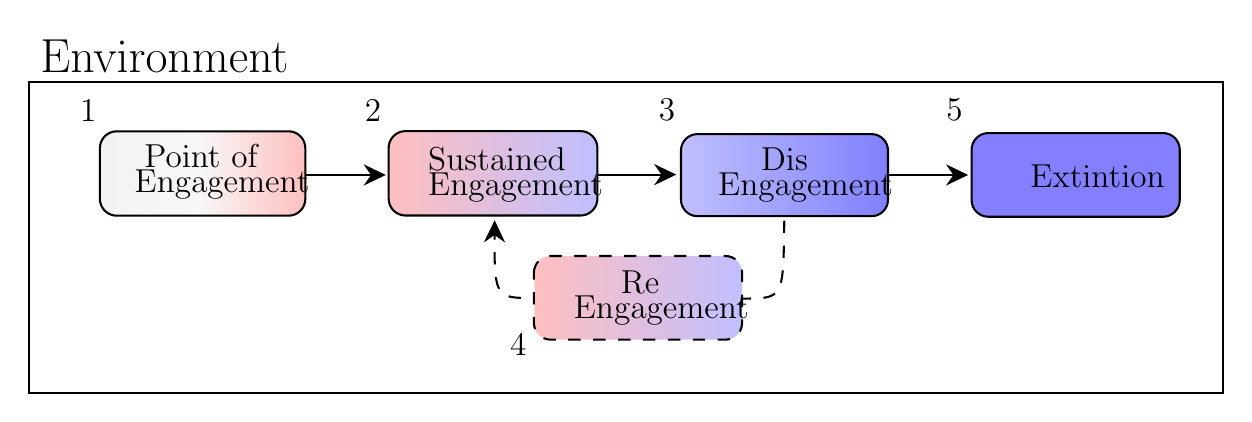
\begin{tikzpicture}[x=0.75pt,y=0.75pt,yscale=-1,xscale=1]
%uncomment if require: \path (0,200); %set diagram left start at 0, and has height of 200

%Shape: Rectangle [id:dp21453085870796063] 
\draw   (14.1,36.6) -- (589.6,36.6) -- (589.6,186.3) -- (14.1,186.3) -- cycle ;
%Rounded Rect [id:dp8669331486657136] 
\path  [shading=_f0h1xn2np,_2yn49zl61,path fading= _gj5ns3oqm ,fading transform={xshift=2}] (48.4,68.36) .. controls (48.4,63.87) and (52.04,60.22) .. (56.53,60.22) -- (139.24,60.22) .. controls (143.73,60.22) and (147.37,63.87) .. (147.37,68.36) -- (147.37,92.76) .. controls (147.37,97.25) and (143.73,100.89) .. (139.24,100.89) -- (56.53,100.89) .. controls (52.04,100.89) and (48.4,97.25) .. (48.4,92.76) -- cycle ; % for fading 
 \draw   (48.4,68.36) .. controls (48.4,63.87) and (52.04,60.22) .. (56.53,60.22) -- (139.24,60.22) .. controls (143.73,60.22) and (147.37,63.87) .. (147.37,68.36) -- (147.37,92.76) .. controls (147.37,97.25) and (143.73,100.89) .. (139.24,100.89) -- (56.53,100.89) .. controls (52.04,100.89) and (48.4,97.25) .. (48.4,92.76) -- cycle ; % for border 

%Straight Lines [id:da4505594811913791] 
\draw    (147.6,81.26) -- (183.16,81.26) ;
\draw [shift={(186.16,81.26)}, rotate = 180] [fill={rgb, 255:red, 0; green, 0; blue, 0 }  ][line width=0.08]  [draw opacity=0] (10.72,-5.15) -- (0,0) -- (10.72,5.15) -- (7.12,0) -- cycle    ;
%Rounded Rect [id:dp29846373438871854] 
\path  [shading=_25n4qjk0b,_5ocf120kv,path fading= _ugfmlo9rg ,fading transform={xshift=2}] (187.51,68.26) .. controls (187.51,63.77) and (191.16,60.13) .. (195.65,60.13) -- (279.95,60.13) .. controls (284.44,60.13) and (288.09,63.77) .. (288.09,68.26) -- (288.09,92.66) .. controls (288.09,97.15) and (284.44,100.8) .. (279.95,100.8) -- (195.65,100.8) .. controls (191.16,100.8) and (187.51,97.15) .. (187.51,92.66) -- cycle ; % for fading 
 \draw   (187.51,68.26) .. controls (187.51,63.77) and (191.16,60.13) .. (195.65,60.13) -- (279.95,60.13) .. controls (284.44,60.13) and (288.09,63.77) .. (288.09,68.26) -- (288.09,92.66) .. controls (288.09,97.15) and (284.44,100.8) .. (279.95,100.8) -- (195.65,100.8) .. controls (191.16,100.8) and (187.51,97.15) .. (187.51,92.66) -- cycle ; % for border 

%Straight Lines [id:da4495263911578298] 
\draw    (288.09,81.1) -- (323.09,81.1) ;
\draw [shift={(326.09,81.1)}, rotate = 180] [fill={rgb, 255:red, 0; green, 0; blue, 0 }  ][line width=0.08]  [draw opacity=0] (10.72,-5.15) -- (0,0) -- (10.72,5.15) -- (7.12,0) -- cycle    ;
%Rounded Rect [id:dp9135925108190124] 
\path  [shading=_03e54ezl1,_daocnbh0q,path fading= _thlshpcj1 ,fading transform={xshift=2}] (328.37,69.49) .. controls (328.37,65.13) and (331.91,61.59) .. (336.28,61.59) -- (420.18,61.59) .. controls (424.55,61.59) and (428.09,65.13) .. (428.09,69.49) -- (428.09,93.21) .. controls (428.09,97.58) and (424.55,101.11) .. (420.18,101.11) -- (336.28,101.11) .. controls (331.91,101.11) and (328.37,97.58) .. (328.37,93.21) -- cycle ; % for fading 
 \draw   (328.37,69.49) .. controls (328.37,65.13) and (331.91,61.59) .. (336.28,61.59) -- (420.18,61.59) .. controls (424.55,61.59) and (428.09,65.13) .. (428.09,69.49) -- (428.09,93.21) .. controls (428.09,97.58) and (424.55,101.11) .. (420.18,101.11) -- (336.28,101.11) .. controls (331.91,101.11) and (328.37,97.58) .. (328.37,93.21) -- cycle ; % for border 

%Rounded Rect [id:dp630049377495355] 
\path  [shading=_qf8n4pbxh,_2e7ef02nx,path fading= _a3543rpu3 ,fading transform={xshift=2}] (257.51,128.36) .. controls (257.51,123.9) and (261.13,120.29) .. (265.58,120.29) -- (349.73,120.29) .. controls (354.19,120.29) and (357.8,123.9) .. (357.8,128.36) -- (357.8,152.55) .. controls (357.8,157.01) and (354.19,160.62) .. (349.73,160.62) -- (265.58,160.62) .. controls (261.13,160.62) and (257.51,157.01) .. (257.51,152.55) -- cycle ; % for fading 
 \draw  [dash pattern={on 4.5pt off 4.5pt}] (257.51,128.36) .. controls (257.51,123.9) and (261.13,120.29) .. (265.58,120.29) -- (349.73,120.29) .. controls (354.19,120.29) and (357.8,123.9) .. (357.8,128.36) -- (357.8,152.55) .. controls (357.8,157.01) and (354.19,160.62) .. (349.73,160.62) -- (265.58,160.62) .. controls (261.13,160.62) and (257.51,157.01) .. (257.51,152.55) -- cycle ; % for border 

%Straight Lines [id:da1505945863891579] 
\draw    (427.92,81.26) -- (463.72,81.26) ;
\draw [shift={(466.72,81.26)}, rotate = 180] [fill={rgb, 255:red, 0; green, 0; blue, 0 }  ][line width=0.08]  [draw opacity=0] (10.72,-5.15) -- (0,0) -- (10.72,5.15) -- (7.12,0) -- cycle    ;
%Rounded Rect [id:dp7652426478992563] 
\draw  [fill={rgb, 255:red, 8; green, 0; blue, 255 }  ,fill opacity=0.5 ] (468.37,69.13) .. controls (468.37,64.68) and (471.98,61.07) .. (476.44,61.07) -- (560.59,61.07) .. controls (565.05,61.07) and (568.66,64.68) .. (568.66,69.13) -- (568.66,93.33) .. controls (568.66,97.79) and (565.05,101.4) .. (560.59,101.4) -- (476.44,101.4) .. controls (471.98,101.4) and (468.37,97.79) .. (468.37,93.33) -- cycle ;
%Curve Lines [id:da6295563644706698] 
\draw  [dash pattern={on 4.5pt off 4.5pt}]  (238.57,106.4) .. controls (238.32,140.92) and (238.67,140.53) .. (257.51,140.53) ;
\draw [shift={(238.6,103.1)}, rotate = 90.44] [fill={rgb, 255:red, 0; green, 0; blue, 0 }  ][line width=0.08]  [draw opacity=0] (10.72,-5.15) -- (0,0) -- (10.72,5.15) -- (7.12,0) -- cycle    ;
%Curve Lines [id:da022545744318036687] 
\draw  [dash pattern={on 4.5pt off 4.5pt}]  (378.14,103.27) .. controls (377.57,140.99) and (378.09,140.81) .. (357.8,140.81) ;

% Text Node
\draw (65.5,23.28) node  [font=\fontsize{0.67em}{0.8em}\selectfont] [align=left] {\begin{minipage}[lt]{68.75pt}\setlength\topsep{0pt}
\begin{center}
{\LARGE Environment}
\end{center}

\end{minipage}};
% Text Node
\draw (97.09,79.56) node  [font=\fontsize{0.67em}{0.8em}\selectfont] [align=left] {\begin{minipage}[lt]{47.87pt}\setlength\topsep{0pt}
\begin{center}
{\large Point of}\\{\large Engagement}
\end{center}

\end{minipage}};
% Text Node
\draw (238.5,80.46) node  [font=\fontsize{0.67em}{0.8em}\selectfont] [align=left] {\begin{minipage}[lt]{47.87pt}\setlength\topsep{0pt}
\begin{center}
{\large Sustained}\\{\large Engagement}
\end{center}

\end{minipage}};
% Text Node
\draw (378.23,81.35) node  [font=\fontsize{0.67em}{0.8em}\selectfont] [align=left] {\begin{minipage}[lt]{47.87pt}\setlength\topsep{0pt}
\begin{center}
{\large Dis}\\{\large Engagement}
\end{center}

\end{minipage}};
% Text Node
\draw (518.51,81.23) node  [font=\fontsize{0.67em}{0.8em}\selectfont] [align=left] {\begin{minipage}[lt]{32.64pt}\setlength\topsep{0pt}
\begin{center}
{\large Extintion}
\end{center}

\end{minipage}};
% Text Node
\draw (308.67,140.46) node  [font=\fontsize{0.67em}{0.8em}\selectfont] [align=left] {\begin{minipage}[lt]{47.87pt}\setlength\topsep{0pt}
\begin{center}
{\large Re}\\{\large Engagement}
\end{center}

\end{minipage}};
% Text Node
\draw (37.33,43.67) node [anchor=north west][inner sep=0.75pt]   [align=left] {{\large 1}};
% Text Node
\draw (174.53,43.67) node [anchor=north west][inner sep=0.75pt]   [align=left] {{\large 2}};
% Text Node
\draw (316.2,43) node [anchor=north west][inner sep=0.75pt]   [align=left] {{\large 3}};
% Text Node
\draw (244.53,156.67) node [anchor=north west][inner sep=0.75pt]   [align=left] {{\large 4}};
% Text Node
\draw (454.73,43) node [anchor=north west][inner sep=0.75pt]   [align=left] {{\large 5}};

\end{tikzpicture}

\end{adjustbox}
\end{center}

\caption[\textbf{Stages of the engagement process mode}]{Solid and dashed lines represent compulsory and  optional paths. Moving from the left to the right we can imagine 1 as being the first interaction that an individual has with an object. This might happen as the result of a prior belief that the object is able to provide a pleasurable experience. The individual will interact with the object for as long as this last one is able to provide a gratifying experience(i.e. stage 2). However, if this is not the case, or constraints from the surrounding environment emerge, the individual will gradually reduce their interaction with the object (i.e. stage 3). At this point we can either observe an alternation between re-engagement and disengagement (i.e. stage 4) or reach an inevitable state of complete withdrawal from the object (i.e. stage 5)}
\label{fig: eng_proc_model_1}
\end{figure}

\paragraph*{Point of engagement} This is the starting point of the engagement process, it is the moment in which the individual’s attention is directed towards a specific object or activity due its properties and capacity to fulfil specific motivational drives.

\paragraph*{Period of engagement} This is the period during which the individual has a sustained interaction with the object of interest. In this case, a situation of sustained and prolonged interaction is conditional on the ability of the object to provide a positive and stimulating experience.

\paragraph*{Disengagement} This stage defines the moment in which the individual reduces the interaction with the object due to internal or external factors. The internal factors are usually connected to loss of interest or pressure derived by the time passing, external factors instead relate more to the inability of the activity to provide a positive experience or to the occurrence of external events in the environment surrounding the individual.

\paragraph*{Re-engagement} It identifies the moment in which the user returns to a sustained level of activity after disengagement occurred. This can happen both in the short and long term and it is the result of positive experiences with the activity, which are usually linked to be exposed to rewarding incentives or novel content within the activity.

\paragraph*{Extinction} In case of prolonged disengagement, marked unsatisfying experiences or impactful external events, the individual might terminate its interactions with the object leaving no further possibility to re-engage with it.

\subsection{From Motivation to Engagement}
\label{eng_reward_motivation}
What emerged from this brief overview of the literature on engagement theories applied to videogames, is that engagement seems to be best described as a process controlled by the characteristics of an object, the internal state of the individual interacting with it and eventual environmental factors external to both. In this view engagement appears as a second order factor generated and derived from the internal state of the individual and concerned with the description and quantification of their interactions with an object  \cite{lucas2004sex,o2008user,jennett2008measuring,boyle2012engagement,connolly2012systematic,csikszentmihalyi2014toward}. The quality and quantity of these interactions seem to be conditional on the ability of the object to provide feelings of enjoyment and pleasure \cite{lucas2004sex,o2008user,jennett2008measuring,boyle2012engagement,connolly2012systematic,csikszentmihalyi2014toward}. For this reason engagement is better understood when framed within a specific context: despite it is generated by processes that are common across any human being (e.g., motivation) its specific connotation is tightly bounded to the characterisitcs of the object of engagement. In other words, engagement can be better understood when framed as \textit{engagement with something} rather than as an abstract entity. 

We can already see a connection between the construct of engagement and the reward-driven motivational processes presented in section \ref{motivation}, especially if we look at the behavioural level. In the context of videogames, motivational processes seem to pertain the formation and modulation of unobservable (i.e., latent) states characterizing the individual before, during and after the interaction with a videogame. On the other hand, engagement appears to describe the observable aspects of this interaction both at the behavioural and experiential level \cite{lucas2004sex,o2008user,jennett2008measuring,boyle2012engagement,connolly2012systematic,csikszentmihalyi2014toward}. A more clear illustration of this idea is presented in Figure \ref{fig: eng_proc_model_2} 

\begin{figure}[h]
\begin{center}
\begin{adjustbox}{width=\columnwidth}

\tikzset {_tol09vz9c/.code = {\pgfsetadditionalshadetransform{ \pgftransformshift{\pgfpoint{0 bp } { 0 bp }  }  \pgftransformrotate{0 }  \pgftransformscale{2 }  }}}
\pgfdeclarehorizontalshading{_j7rsmr3nr}{150bp}{rgb(0bp)=(0.93,0.93,0.93);
rgb(37.5bp)=(0.93,0.93,0.93);
rgb(62.5bp)=(1,0,0);
rgb(100bp)=(1,0,0)}
\tikzset{_yxq6cdpsj/.code = {\pgfsetadditionalshadetransform{\pgftransformshift{\pgfpoint{0 bp } { 0 bp }  }  \pgftransformrotate{0 }  \pgftransformscale{2 } }}}
\pgfdeclarehorizontalshading{_7yg524gtp} {150bp} {color(0bp)=(transparent!75);
color(37.5bp)=(transparent!75);
color(62.5bp)=(transparent!75);
color(100bp)=(transparent!75) } 
\pgfdeclarefading{_y4z1b8bbb}{\tikz \fill[shading=_7yg524gtp,_yxq6cdpsj] (0,0) rectangle (50bp,50bp); } 

% Gradient Info
  
\tikzset {_3ywdqyfah/.code = {\pgfsetadditionalshadetransform{ \pgftransformshift{\pgfpoint{0 bp } { 0 bp }  }  \pgftransformrotate{0 }  \pgftransformscale{2 }  }}}
\pgfdeclarehorizontalshading{_2t0kw1fpw}{150bp}{rgb(0bp)=(1,0,0);
rgb(37.5bp)=(1,0,0);
rgb(62.5bp)=(0,0,1);
rgb(100bp)=(0,0,1)}
\tikzset{_yvsljnreh/.code = {\pgfsetadditionalshadetransform{\pgftransformshift{\pgfpoint{0 bp } { 0 bp }  }  \pgftransformrotate{0 }  \pgftransformscale{2 } }}}
\pgfdeclarehorizontalshading{_fpvhgjdei} {150bp} {color(0bp)=(transparent!75);
color(37.5bp)=(transparent!75);
color(62.5bp)=(transparent!75);
color(100bp)=(transparent!75) } 
\pgfdeclarefading{_y32y00acn}{\tikz \fill[shading=_fpvhgjdei,_yvsljnreh] (0,0) rectangle (50bp,50bp); } 

% Gradient Info
  
\tikzset {_k82gbaai2/.code = {\pgfsetadditionalshadetransform{ \pgftransformshift{\pgfpoint{0 bp } { 0 bp }  }  \pgftransformrotate{0 }  \pgftransformscale{2 }  }}}
\pgfdeclarehorizontalshading{_mzd6axxaa}{150bp}{rgb(0bp)=(0,0,1);
rgb(37.5bp)=(0,0,1);
rgb(62.5bp)=(0,0,1);
rgb(100bp)=(0,0,1)}
\tikzset{_1ih9fwhej/.code = {\pgfsetadditionalshadetransform{\pgftransformshift{\pgfpoint{0 bp } { 0 bp }  }  \pgftransformrotate{0 }  \pgftransformscale{2 } }}}
\pgfdeclarehorizontalshading{_py52u7ab2} {150bp} {color(0bp)=(transparent!75);
color(37.5bp)=(transparent!75);
color(62.5bp)=(transparent!50);
color(100bp)=(transparent!50) } 
\pgfdeclarefading{_wr0vkxl3y}{\tikz \fill[shading=_py52u7ab2,_1ih9fwhej] (0,0) rectangle (50bp,50bp); } 

% Gradient Info
  
\tikzset {_3kvg59946/.code = {\pgfsetadditionalshadetransform{ \pgftransformshift{\pgfpoint{0 bp } { 0 bp }  }  \pgftransformrotate{-90 }  \pgftransformscale{2 }  }}}
\pgfdeclarehorizontalshading{_wvh4fdo7p}{150bp}{rgb(0bp)=(1,0,0);
rgb(37.5bp)=(1,0,0);
rgb(62.5bp)=(0,0,1);
rgb(100bp)=(0,0,1)}
\tikzset{_dv8t3n3dv/.code = {\pgfsetadditionalshadetransform{\pgftransformshift{\pgfpoint{0 bp } { 0 bp }  }  \pgftransformrotate{-90 }  \pgftransformscale{2 } }}}
\pgfdeclarehorizontalshading{_abfcxja44} {150bp} {color(0bp)=(transparent!75);
color(37.5bp)=(transparent!75);
color(62.5bp)=(transparent!75);
color(100bp)=(transparent!75) } 
\pgfdeclarefading{_tndnn1d2b}{\tikz \fill[shading=_abfcxja44,_dv8t3n3dv] (0,0) rectangle (50bp,50bp); } 

% Gradient Info
  
\tikzset {_475pso13i/.code = {\pgfsetadditionalshadetransform{ \pgftransformshift{\pgfpoint{0 bp } { 0 bp }  }  \pgftransformrotate{-90 }  \pgftransformscale{2 }  }}}
\pgfdeclarehorizontalshading{_f5gjc5tzr}{150bp}{rgb(0bp)=(0,0,1);
rgb(37.5bp)=(0,0,1);
rgb(62.5bp)=(1,0,0);
rgb(100bp)=(1,0,0)}
\tikzset{_fwuteqqte/.code = {\pgfsetadditionalshadetransform{\pgftransformshift{\pgfpoint{0 bp } { 0 bp }  }  \pgftransformrotate{-90 }  \pgftransformscale{2 } }}}
\pgfdeclarehorizontalshading{_gbjam9yyh} {150bp} {color(0bp)=(transparent!75);
color(37.5bp)=(transparent!75);
color(62.5bp)=(transparent!75);
color(100bp)=(transparent!75) } 
\pgfdeclarefading{_wo5obn5gu}{\tikz \fill[shading=_gbjam9yyh,_fwuteqqte] (0,0) rectangle (50bp,50bp); } 
\tikzset{every picture/.style={line width=0.75pt}} %set default line width to 0.75pt        

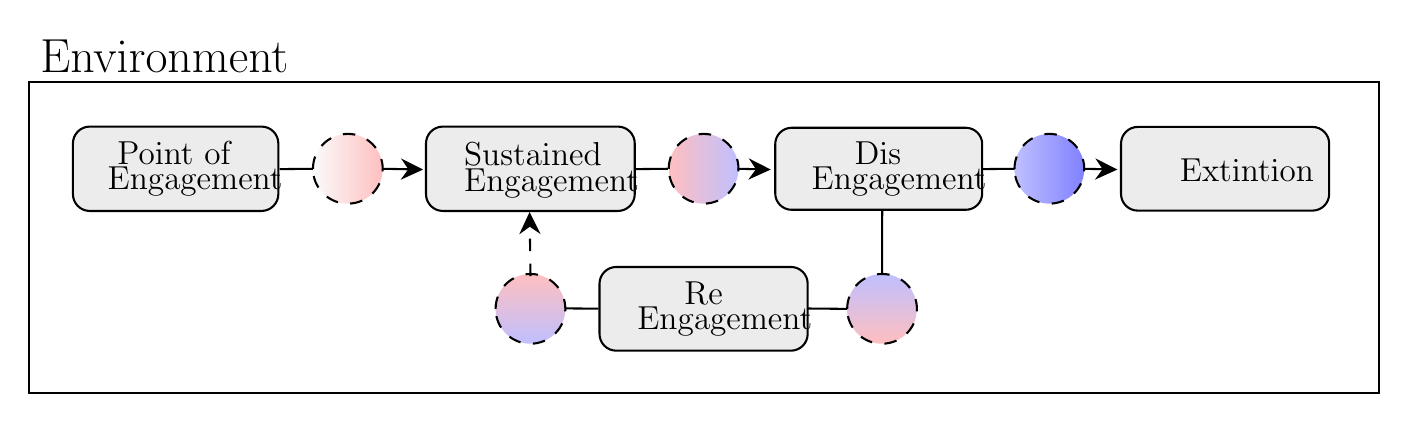
\begin{tikzpicture}[x=0.75pt,y=0.75pt,yscale=-1,xscale=1]
%uncomment if require: \path (0,357); %set diagram left start at 0, and has height of 357

%Rounded Rect [id:dp08887598870261693] 
\draw  [fill={rgb, 255:red, 236; green, 236; blue, 236 }  ,fill opacity=1 ] (30.4,81.08) .. controls (30.4,76.59) and (34.04,72.95) .. (38.53,72.95) -- (121.24,72.95) .. controls (125.73,72.95) and (129.37,76.59) .. (129.37,81.08) -- (129.37,105.48) .. controls (129.37,109.97) and (125.73,113.61) .. (121.24,113.61) -- (38.53,113.61) .. controls (34.04,113.61) and (30.4,109.97) .. (30.4,105.48) -- cycle ;
%Rounded Rect [id:dp06222122397376195] 
\draw  [fill={rgb, 255:red, 236; green, 236; blue, 236 }  ,fill opacity=1 ] (200.51,81.08) .. controls (200.51,76.59) and (204.16,72.95) .. (208.65,72.95) -- (292.95,72.95) .. controls (297.44,72.95) and (301.09,76.59) .. (301.09,81.08) -- (301.09,105.48) .. controls (301.09,109.97) and (297.44,113.61) .. (292.95,113.61) -- (208.65,113.61) .. controls (204.16,113.61) and (200.51,109.97) .. (200.51,105.48) -- cycle ;
%Rounded Rect [id:dp7821816318063516] 
\draw  [fill={rgb, 255:red, 236; green, 236; blue, 236 }  ,fill opacity=1 ] (368.77,81.42) .. controls (368.77,77.06) and (372.31,73.52) .. (376.68,73.52) -- (460.58,73.52) .. controls (464.95,73.52) and (468.49,77.06) .. (468.49,81.42) -- (468.49,105.14) .. controls (468.49,109.5) and (464.95,113.04) .. (460.58,113.04) -- (376.68,113.04) .. controls (372.31,113.04) and (368.77,109.5) .. (368.77,105.14) -- cycle ;
%Rounded Rect [id:dp20372970008362923] 
\draw  [fill={rgb, 255:red, 236; green, 236; blue, 236 }  ,fill opacity=1 ] (535.37,81.18) .. controls (535.37,76.73) and (538.98,73.12) .. (543.44,73.12) -- (627.59,73.12) .. controls (632.05,73.12) and (635.66,76.73) .. (635.66,81.18) -- (635.66,105.38) .. controls (635.66,109.83) and (632.05,113.44) .. (627.59,113.44) -- (543.44,113.44) .. controls (538.98,113.44) and (535.37,109.83) .. (535.37,105.38) -- cycle ;
%Shape: Circle [id:dp19552380180112794] 
\path  [shading=_j7rsmr3nr,_tol09vz9c,path fading= _y4z1b8bbb ,fading transform={xshift=2}] (146.05,93.28) .. controls (146.05,84) and (153.57,76.48) .. (162.85,76.48) .. controls (172.13,76.48) and (179.65,84) .. (179.65,93.28) .. controls (179.65,102.56) and (172.13,110.08) .. (162.85,110.08) .. controls (153.57,110.08) and (146.05,102.56) .. (146.05,93.28) -- cycle ; % for fading 
 \draw  [dash pattern={on 4.5pt off 4.5pt}] (146.05,93.28) .. controls (146.05,84) and (153.57,76.48) .. (162.85,76.48) .. controls (172.13,76.48) and (179.65,84) .. (179.65,93.28) .. controls (179.65,102.56) and (172.13,110.08) .. (162.85,110.08) .. controls (153.57,110.08) and (146.05,102.56) .. (146.05,93.28) -- cycle ; % for border 

%Shape: Circle [id:dp27430889542654724] 
\path  [shading=_2t0kw1fpw,_3ywdqyfah,path fading= _y32y00acn ,fading transform={xshift=2}] (317.46,93.28) .. controls (317.46,84) and (324.98,76.48) .. (334.26,76.48) .. controls (343.54,76.48) and (351.06,84) .. (351.06,93.28) .. controls (351.06,102.56) and (343.54,110.08) .. (334.26,110.08) .. controls (324.98,110.08) and (317.46,102.56) .. (317.46,93.28) -- cycle ; % for fading 
 \draw  [dash pattern={on 4.5pt off 4.5pt}] (317.46,93.28) .. controls (317.46,84) and (324.98,76.48) .. (334.26,76.48) .. controls (343.54,76.48) and (351.06,84) .. (351.06,93.28) .. controls (351.06,102.56) and (343.54,110.08) .. (334.26,110.08) .. controls (324.98,110.08) and (317.46,102.56) .. (317.46,93.28) -- cycle ; % for border 

%Rounded Rect [id:dp4578454458037269] 
\draw  [fill={rgb, 255:red, 236; green, 236; blue, 236 }  ,fill opacity=1 ] (284.11,148.66) .. controls (284.11,144.2) and (287.73,140.59) .. (292.18,140.59) -- (376.33,140.59) .. controls (380.79,140.59) and (384.4,144.2) .. (384.4,148.66) -- (384.4,172.85) .. controls (384.4,177.31) and (380.79,180.92) .. (376.33,180.92) -- (292.18,180.92) .. controls (287.73,180.92) and (284.11,177.31) .. (284.11,172.85) -- cycle ;
%Shape: Circle [id:dp8141702965644008] 
\path  [shading=_mzd6axxaa,_k82gbaai2,path fading= _wr0vkxl3y ,fading transform={xshift=2}] (484.05,93.28) .. controls (484.05,84) and (491.57,76.48) .. (500.85,76.48) .. controls (510.13,76.48) and (517.65,84) .. (517.65,93.28) .. controls (517.65,102.56) and (510.13,110.08) .. (500.85,110.08) .. controls (491.57,110.08) and (484.05,102.56) .. (484.05,93.28) -- cycle ; % for fading 
 \draw  [dash pattern={on 4.5pt off 4.5pt}] (484.05,93.28) .. controls (484.05,84) and (491.57,76.48) .. (500.85,76.48) .. controls (510.13,76.48) and (517.65,84) .. (517.65,93.28) .. controls (517.65,102.56) and (510.13,110.08) .. (500.85,110.08) .. controls (491.57,110.08) and (484.05,102.56) .. (484.05,93.28) -- cycle ; % for border 

%Shape: Circle [id:dp5389996328417695] 
\path  [shading=_wvh4fdo7p,_3kvg59946,path fading= _tndnn1d2b ,fading transform={xshift=2}] (234.05,160.76) .. controls (234.05,151.48) and (241.57,143.96) .. (250.85,143.96) .. controls (260.13,143.96) and (267.65,151.48) .. (267.65,160.76) .. controls (267.65,170.03) and (260.13,177.56) .. (250.85,177.56) .. controls (241.57,177.56) and (234.05,170.03) .. (234.05,160.76) -- cycle ; % for fading 
 \draw  [dash pattern={on 4.5pt off 4.5pt}] (234.05,160.76) .. controls (234.05,151.48) and (241.57,143.96) .. (250.85,143.96) .. controls (260.13,143.96) and (267.65,151.48) .. (267.65,160.76) .. controls (267.65,170.03) and (260.13,177.56) .. (250.85,177.56) .. controls (241.57,177.56) and (234.05,170.03) .. (234.05,160.76) -- cycle ; % for border 

%Shape: Circle [id:dp655926787503073] 
\path  [shading=_f5gjc5tzr,_475pso13i,path fading= _wo5obn5gu ,fading transform={xshift=2}] (403.43,160.76) .. controls (403.43,151.48) and (410.95,143.96) .. (420.23,143.96) .. controls (429.51,143.96) and (437.03,151.48) .. (437.03,160.76) .. controls (437.03,170.03) and (429.51,177.56) .. (420.23,177.56) .. controls (410.95,177.56) and (403.43,170.03) .. (403.43,160.76) -- cycle ; % for fading 
 \draw  [dash pattern={on 4.5pt off 4.5pt}] (403.43,160.76) .. controls (403.43,151.48) and (410.95,143.96) .. (420.23,143.96) .. controls (429.51,143.96) and (437.03,151.48) .. (437.03,160.76) .. controls (437.03,170.03) and (429.51,177.56) .. (420.23,177.56) .. controls (410.95,177.56) and (403.43,170.03) .. (403.43,160.76) -- cycle ; % for border 

%Shape: Rectangle [id:dp8053989914309859] 
\draw   (9.1,51.6) -- (659.6,51.6) -- (659.6,201.3) -- (9.1,201.3) -- cycle ;
%Straight Lines [id:da46348057228029615] 
\draw    (130,93.45) -- (146.05,93.28) ;
%Straight Lines [id:da06616438858203633] 
\draw    (179.65,93.28) -- (196.1,93.59) ;
\draw [shift={(199.1,93.65)}, rotate = 181.09] [fill={rgb, 255:red, 0; green, 0; blue, 0 }  ][line width=0.08]  [draw opacity=0] (10.72,-5.15) -- (0,0) -- (10.72,5.15) -- (7.12,0) -- cycle    ;
%Straight Lines [id:da6977755883492565] 
\draw    (350.65,93.28) -- (363.6,93.58) ;
\draw [shift={(366.6,93.65)}, rotate = 181.33] [fill={rgb, 255:red, 0; green, 0; blue, 0 }  ][line width=0.08]  [draw opacity=0] (10.72,-5.15) -- (0,0) -- (10.72,5.15) -- (7.12,0) -- cycle    ;
%Straight Lines [id:da47311877150256343] 
\draw    (301,93.45) -- (317.05,93.28) ;
%Straight Lines [id:da21451072469562127] 
\draw    (468,93.45) -- (484.05,93.28) ;
%Straight Lines [id:da7997515132020875] 
\draw    (517.65,93.28) -- (530.6,93.58) ;
\draw [shift={(533.6,93.65)}, rotate = 181.33] [fill={rgb, 255:red, 0; green, 0; blue, 0 }  ][line width=0.08]  [draw opacity=0] (10.72,-5.15) -- (0,0) -- (10.72,5.15) -- (7.12,0) -- cycle    ;
%Straight Lines [id:da5942266070774226] 
\draw    (420.23,143.98) -- (420.32,112.84) ;
%Straight Lines [id:da1853788628800106] 
\draw  [dash pattern={on 4.5pt off 4.5pt}]  (250.85,144.98) -- (250.47,117.1) ;
\draw [shift={(250.42,114.1)}, rotate = 89.2] [fill={rgb, 255:red, 0; green, 0; blue, 0 }  ][line width=0.08]  [draw opacity=0] (10.72,-5.15) -- (0,0) -- (10.72,5.15) -- (7.12,0) -- cycle    ;
%Straight Lines [id:da47123825108915496] 
\draw    (403.43,160.78) -- (384.32,160.6) ;
%Straight Lines [id:da3253725947262416] 
\draw    (283.52,160.68) -- (267.65,160.55) ;

% Text Node
\draw (334.26,160.76) node  [font=\fontsize{0.67em}{0.8em}\selectfont] [align=left] {\begin{minipage}[lt]{47.87pt}\setlength\topsep{0pt}
\begin{center}
{\large Re}\\{\large Engagement}
\end{center}

\end{minipage}};
% Text Node
\draw (79.09,93.28) node  [font=\fontsize{0.67em}{0.8em}\selectfont] [align=left] {\begin{minipage}[lt]{47.87pt}\setlength\topsep{0pt}
\begin{center}
{\large Point of}\\{\large Engagement}
\end{center}

\end{minipage}};
% Text Node
\draw (60.5,38.28) node  [font=\fontsize{0.67em}{0.8em}\selectfont] [align=left] {\begin{minipage}[lt]{68.75pt}\setlength\topsep{0pt}
\begin{center}
{\LARGE Environment}
\end{center}

\end{minipage}};
% Text Node
\draw (418.23,93.28) node  [font=\fontsize{0.67em}{0.8em}\selectfont] [align=left] {\begin{minipage}[lt]{47.87pt}\setlength\topsep{0pt}
\begin{center}
{\large Dis}\\{\large Engagement}
\end{center}

\end{minipage}};
% Text Node
\draw (585.51,93.28) node  [font=\fontsize{0.67em}{0.8em}\selectfont] [align=left] {\begin{minipage}[lt]{32.64pt}\setlength\topsep{0pt}
\begin{center}
{\large Extintion}
\end{center}

\end{minipage}};
% Text Node
\draw (250.8,93.28) node  [font=\fontsize{0.67em}{0.8em}\selectfont] [align=left] {\begin{minipage}[lt]{47.87pt}\setlength\topsep{0pt}
\begin{center}
{\large Sustained}\\{\large Engagement}
\end{center}

\end{minipage}};
\end{tikzpicture}

\end{adjustbox}
\end{center}
\caption{\textbf{Diagram summarizing the different stages of the engagement process mode introducing the contribution of environment and latent states}.}
\label{fig: eng_proc_model_2}
\end{figure}

Here we adapted the engagement process model of O'Brien and colleagues \cite{o2008user} presented in Figure \ref{fig: eng_proc_model_1} incorporating the state of the individual. In this view, the motivational state of an individual precede (on an arbitrary temporal scale) and contribute at determining in which phase of the engagement process an individual will be located when interacting with as specific object (i.e., a videogame) again in the future. This implies that, at any point in time, the history of observed engagement indicators (e.g., frequency and amount of interactions) can provide information on the current unobservable motivational state of the individual. 

In section \ref{motivation_hist} we specified that the motivational propensity that an individual might have towards a certain object is in part determined by the rewarding properties of the object itself \cite{berridge2004motivation}. But how would these properties look in the context of a videogame? Surely playing videogames is not relevant for satisfying fundamental physiological needs nor it is directly linked to other type of powerful reinforcers (e.g. money). In this case, the distinction between primary and secondary rewards made in section \ref{motivation_hist} becomes particularly useful for understating the framework in which videogames lies: what acts as a reinforcer during the playing behaviour are the structural characteristics defining the videogame itself \cite{king2010role, king2010video, yannakakis2013player}. We will better define the concept of videogame structural characteristics later on but for now we can think of them as any type of in-game element that an individual might interact with during the playing behaviour \cite{king2010role,king2010video}. None of these structural characteristics are intrinsically rewarding, but they can become so over time, through conventional learning processes, if they are able to provide pleasurable experiences to the individual \cite{skinner1953science, berridge2004motivation, przybylski2010motivational}. In a dynamic fashion, interacting with specific features in the videogame might produce positive reactions in the individual and make new interactions more probable. 

In this view engagement can be seen as the observable manifestation of the unobservable motivational propensity that an individual has towards a specific videogame. In other words, we can think of engagement as the behavioural realisation of a motivational process aimed at maximizing the positive experiences provided by the in-game elements. 

\subsection{Videogames Structural Characteristics}
\label{factors_engagement}
It should be evident by now that the ability to construct videogames with effective rewarding characteristics is of pivotal importance for generating and sustaining engagement \cite{king2010role, king2010video, yannakakis2013player}. 

Various attempt has been made to build a taxonomy of these characteristics, King et al. \cite{king2010video} for instance outlined a series of features that effective videogames structural characteristics should have. These are: social features, manipulation (e.g. crafting) features, narrative features, achievement and punishing features and aesthetic features. Westwood et al. \cite{westwood2010role} were able to use this taxonomy for effectively individuating which specific structural characteristic were driving playing behaviour in a group of videogame players. The taxonomy provided by King et al. \cite{king2010video}, although exhaustive, provides a descriptive rather than mechanistic account of the structural characteristic driving playing behaviour \cite{king2010role}. Adopting a different approach, Wang and Sun proposed to frame the work of King et al. in terms of reinforcers \cite{king2010video, wang2011game}. In this view, playing behaviour in different games is sustained by different reinforcing mechanics covering the areas described by King et al. \cite{king2010video, wang2011game}. Among these mechanics there are: scoring systems, in-game items and resources, achievements systems, feedback messages, animation events and the unlocking of new game contents \cite{wang2011game}. The authors also described a series of attributes that the in-game rewards should have for being effective: they need to possess social value within a shared environment, they need to have visible effects within the game world and they need time and effort to be obtained \cite{wang2011game}. Extending the work of Wang and Sun, Philips and colleagues focused on a description of the temporal characteristics that in-game reinforcers may possess, namely being limited in duration, transient and context dependent, permanent or consumable \cite{phillips2013videogame}. 

A connected although separate stream of research tried to categorize which elements inside a videogame might produce pleasurable experiences for the players however focusing more on the characteristics of the individuals rather than those of the game itself. Similarly to trait theories in psychology, this approach assume that different individual have static, consistent and well defined preferences for some aspects (i.e. structural characteristics). of the playing experience. In his seminal work Bartle tried to identify different approaches that players might have had in playing Multi User Dungeons (MUDs), an early version of the modern Massively Multiplayer Online Role Playing Games (MMORPGs) \cite{bartle1996hearts}. Projecting the players’ attitudes towards the game on two axis: oriented towards action or interaction and oriented towards the game world or the players, Bartle proposed four mutually exclusive categories \cite{bartle1996hearts}.

\begin{table}[h]
\caption{\textbf{Bartle Taxonomy}}
\label{bartle}
\begin{tabularx}{\textwidth}{|l|X|}
\hline
Achievers   & Action oriented towards the game world. Players interested in mastering the game, aiming to build a status within the game towards their interaction with the environment.                      \\ \hline
Socializers & Interaction with other players. Players driven by the perspective of interacting with other players, deriving satisfaction from their friendship, contacts and social influence within the game \\ \hline
Explorers   & Interaction with the game world. Players aiming to be surprised by the game world, seeking the stimulation derived by the discovery of new areas and the acquisition of knowledge.              \\ \hline
Killers     & Action oriented towards other players. Players interested in demonstrating their superiority over other players posing great value on the reputation obtained through in-game fighting skills.  \\ \hline
\end{tabularx}
\end{table}

Despite this early formulation only considers a specific subset of games and lacks any kind of empirical validation, Bartle's work was the starting point for most of the later efforts on the subject \cite{bartle1996hearts}. Bartle's taxonomy was built on assumptions that were never tested and the proposed categories showed a certain degree of inter-correlation. For this reason Yee tried to develop a methodology for assessing the players’ tendencies towards specific game characteristics \cite{yee2006motivations}. After gathering information from a large sample of players and performing a first round of dimensionality reduction, 10 major factors emerged, these were then condensed in 3 additional facets performing an ulterior round of dimensionality reduction over the previously obtained components \cite{yee2006motivations}. The three main factors that emerged were: 

\begin{table}[h]
\caption{\textbf{Yee Taxonomy}}
\label{yee}
\begin{tabularx}{\textwidth}{|l|X|}
\hline
Achievement & Factor indicating a tendency towards advancing in the game, exploiting its mechanics or competing with it.                           \\ \hline
Social      & Factor indicating a preference for those game characteristics centred on socializing, creating relationship and developing teamwork. \\ \hline
Immersion   & Factor  represents the drive towards the discovery, role-playing and customization mechanics of the game.                            \\ \hline
\end{tabularx}
\end{table}

The model proposed by Yee introduced two interesting variations on what has been done by Bartle: the components are not necessarily mutually exclusive and the focus is shifted from a characterization of the players to a characterization of the in-game elements with which the individuals interact \cite{bartle1996hearts,yee2006motivations}. Despite these improvements, the focus was still on a specific game genre and heavily relied on static and potentially biased measures (i.e. self-report). In order to overcome the limitations of a taxonomy heavily influenced by a specific game genre, Nacke et al. developed a more comprehensive system with the intent to capture the players’ preferences for particular game mechanics regardless of the genre \cite{nacke2011brainhex}. The categories proposed by this model were: 

\begin{table}[h]
\caption{\textbf{BrainHex Taxonomy}}
\label{nacke}
\begin{tabularx}{\textwidth}{|l|X|}
\hline
Seekers     & Players driven by in game mechanics which produces interest and satisfy curiosity..                                                    \\ \hline
Daredevils  & Players motivated by the thrill derived from taking risks in the game.                                                                 \\ \hline
Masterminds & Players who enjoys solving puzzles and finding the best strategies to adopt within the game.                                           \\ \hline
Conquerors  & Players who derive satisfaction from overcoming the challenges provided by the game and from the struggles characterizing the process. \\ \hline
Socializers & Players driven by the interaction with other players.                                                                                  \\ \hline
Achievers   & Players driven by reaching long term goals, often aiming to fully complete the game.                                                   \\ \hline
Survivors   & Players driven by thrilling experiences provided by the game and by the ability of the game environment to generate arousal.           \\ \hline
\end{tabularx}
\end{table}

This formulation appear to have a higher level of details than the approaches of Yee and Bartle, however the number of considered factors grows proportional with the number of game characteristics taken into consideration \cite{nacke2011brainhex}. We won't expand on the supposed link between facets, "neurobiology" and personality components proposed by the authors. The first is purely anecdotal, not supported by any evidence and adopt a conceptualization of the human brain that is, at the very least, primitive (reminiscent of the phrenologist Franz Joseph Gall \cite{gall1835functions})\cite{nacke2011brainhex}. Evaluating the relationship between the facets and personality traits could have been an interesting angle to explore, but the use of the infamous Mayers-Briggs model of personality \cite{boyle1995myers} makes the results hard to interpret. 

Differently from most taxonomies presented so far, which are specific to the videogame literature, the work of Przybylski and colleagues leverage the self determination theory of Rayan and Deci \cite{ryan2000self,ryan2006motivational}, a socio-psychological theory of  motivation, for explaining in an empirical way the process through which videogames drive sustained engagement \cite{przybylski2010motivational}. The original work by Ryan and Deci states that humans are driven in their every-day life by the satisfaction of basic needs which are more effective motivational factors than any kind of  external incentive \cite{ryan2000self,ryan2006motivational}. These basic needs are radically different from the physiological one presented in section \ref{motivation} and pertain the need for competence, autonomy, relatedness and control. On the other side, the external incentive mentioned by the theory are closely related to the concept of reinforcers presented in section \ref{motivation_hist}. Ryan and Deci make a distinction between intrinsically motivated behaviours (behaviours motivated by the satisfaction of one of the aforementioned fundamental needs) and extrinsically motivated ones (behaviours motivated by reinforcers coming from the environment like money or tokens). In this view, Przybylski and colleagues proposed that videogames, lacking the presence of external reinforcers, provide appeal via the inherent properties of the playing experience \cite{przybylski2010motivational}. If a videogame is able, through its structural characteristics, to satisfy the individual in one or more of the four fundamental dimension mentioned before it will also be able to promote a state of sustained engagement \cite{przybylski2010motivational}.

\begin{table}[h]
\caption{\textbf{Self-Determination Taxonomy}}
\label{deci}
\begin{tabularx}{\textwidth}{|l|X|}
\hline
Competence  & The satisfaction of this need can be provided by the optimal balance between game difficulty and player skill. The player should never be bored or overwhelmed by the game instead should feel competent while playing.  \\ \hline
Autonomy    & The satisfaction of this need can be provided allowing the player to advance through different challenges and shape the game world in accordance to their will, allowing them to act with freedom within the game.       \\ \hline
Relatedness & The satisfaction of this need can be achieved though social interactions within the game.                                                                                                                                \\ \hline
Control     & The satisfaction of this need can be achieved allowing the player to master the controls of the game putting them in the position of experiencing a sense of control and receiving appropriated feedbacks from the game. \\ \hline
\end{tabularx}
\end{table}

One of the core idea behind the work of Przybylski et al. is that when the playing activity is focused on obtaining reinforcers and avoiding punishments it fosters extrinsic motivation, with potential negative effect on engagement \cite{przybylski2010motivational}.  

Despite the effort made for creating a connection between psychology and the literature on videogames, we found the work of Przybylski et al. to fall short in reconciliating with a long experimental tradition highlighting the pivotal role of (relevant) reinforcers in shaping and driving motivation at the behavioural, cognitive and affective level \cite{skinner1953science,schultz1997neural,berridge2004motivation}. Moreover, a less scientific but potentially more evident proof of the limitation of applying Ryan and Deci theory for understanding the motivational drive of videogames is the staggering success of titles heavily and explicitly relying on reinforcement and punishment mechanisms \cite{darksouls,candyc}. We will not go into the merit of arguing if self determination theory is an appropriate approximation of motivational processes in humans, but what we can highlight how its application to the videogame context seems to be more appropriate for describing issues related to usability and only tangentially relevant for describing the motivational drive of videogames.

In summary we could say that each videogame can be considered as an object with particular structural characteristics (i.e., in-game features) and rules (i.e., games mechanics). Individuals purposely decide to interact with these objects without any (in most cases) requirement from the external world (again, playing game in most cases is not necessary for our survival nor is mandate by any societal norm). What drives these interactions are solely the characteristics of the game that if able to provide a pleasurable experience in a particular point in time will promote more interactions between the individual and the game object. 

We have seen how there is no real consensus in the literature over a specific taxonomy describing the structural characteristics underlying the motivational drive offered by videogames, however some common themes seem to emerge. A structural characteristic acts as a reinforcer if it is able to generate positive reactions in the player. At any given point in time, the game feature with which an individual interact the most can be seen as a promising candidate for the role of motivational driver (i.e., reinforcer). A common set of characteristics and facets that could act as reinforcers seem to emerge across the works presented so far, namely: achievement, socialization, exploration and fighting. However, this might be an artefact created by the fact that most taxonomies appear to have the work of Bartle as a common ancestor \cite{bartle1996hearts,yee2006motivations,nacke2011brainhex}. 

In conclusion, we can say that the lack of a general and unified theory defining how videogames produce motivated behaviour (reads engagement) might be the result of various factors. One, a particular attention for holistic descriptions of the experiential aspects of engagement rather than its mechanistic functioning. Two, a strong focus on producing (relatively game specific) taxonomies of videogames structural characteristics rather than a general theory deriving how these contribute to control engagement. Three, a disconnect between theories of engagement in a videogame setting and robust psychological and neuroscientific constructs (e.g. motivation). In this view, trying to understand engagement through the lenses of well established theories of motivation might provide us with a unifying framework for making sense and better oprationalize the set of heterogeneous evidence that we presented so fa.

\section{Measuring Engagement and Motivation}
\label{measuring_motivation_engagement}
In the previous section we proposed the idea of engagement being the observable realization of latent states generated by those psychological processes controlling the interactions between individuals and videogames. This implies that differently from constructs like motivational states it should be easier to derive quantitative and qualitative measures of the amount and direction of engagement. We report here three different approaches, with their relative strengths and weaknesses, for the measurement of engagement (in particular withing a videogame setting).

\subsection{Self-report Measures}
\label{self_report}
These measures include all those techniques requiring individuals to report their experiences and personal, psychological or demographic characteristics usually with the aim of measuring static/stable attributes. 

Most of the time the measurement is carried out through questionnaires constructed to reliably measure a common construct. Examples used for gathering measures of motivational propensity are the BIS-BAS scale \cite{carver1994behavioral}, focusing on assessing the responsiveness to incentives, or the many different questionnaires developed for measuring the constructs of intrinsic and extrinsic motivation proposed by Ryan and Deci \cite{ryan2000self}. 

The advantages provided by these measures can be found in their relative simplicity, easiness of use, scalability and possibility to simultaneously investigate large sets of constructs. 

That said, they are not exempt from limitations: questionnaires often require the cognitive appraisal of actions, emotions or attitudes. This is an important component for a questionnaire to be effective, nevertheless individuals are not always aware (or able to retrieve and precisely describe) of the motives behind a set of actions or emotional responses \cite{avserivskis2017computational}. Indeed we must stress that conscious appraisal and actual experience may interact and overlap but often do not coincide \cite{poeller2018let}. 

This is supported by the fact that despite many attempts has been carried out for finding an associations between in-game behaviour and self-report measures the findings has often resulted fragmented, inconsistent or inconclusive \cite{canossa2013give, stankevicius2015factor, schaekermann2017curiously}. For example, in a work by Van Lankveld and colleagues \cite{van2009psychologically} the authors investigated the relationship between a large number of behavioural metrics (derived from the interaction of 44 participants with a game) and the score to the NEO-PI-R (a questionnaire for the evaluation of the five-factor model of personality) \cite{costa2008revised}. The results highlighted multiple, but a-specific, correlational patterns. Following this approach, Canossa and colleagues \cite{canossa2013give} also tried to investigate the relationship between self-report measures of psychological characteristics and gaming behaviour however in a larger sample. The results were similar to the work of Van Lankveld et al. in the sense that in-game behaviours appeared to relate with various psychological traits but the underlying meaning of this relationships was hard to derive. In another work by Lankveld et al. the authors narrowed the focus on a single personality trait (i.e. extraversion)  and specifically designed a short game for retrieving behavioural metrics supposedly able to mirror the specific constructs under investigation. Although promising the results can be regarded as borderline inconclusive (i.e., of the 26 in-games metrics considered only 5 showed to be related with the construct of extraversion) \cite{van2011games}. 

One reason for these unsatisfactory results might reside in the nature of the employed questionnaire: conventional psychometric measures have not been developed for describing an individual's behaviour withing a digital setting \cite{yannakakis2013player}. Ad-hoc questionnaires have been developed for measuring game specific constructs \cite{yee2006motivations,tondello2016gamification}, but differently from their psychological counterpart they often seem to not rely on extensive validation procedures. A series of other limitations can be found in the adoption of self report measures, namely: the adherence of the respondents to social desirability norms, erroneous interpretation of the questions, untruthful answers, constrains in the possible answers, random or systematic measurement errors and in case of mass administrations (i.e., mailing or online recruiting) poor sampling control \cite{van2009psychologically}.

\subsection{Psychophysiological Measures}
\label{psychophisio} 
As we mentioned in section \ref{self_report}, self-report methods aim to measure a latent construct, be it a trait or a state, through a series of questions. This quantification is by definition static and, as we mentioned before, relatively prone to bias or systematic measurement errors \cite{van2009psychologically}. 

On the opposite side of the spectrum we can find those measures acquired through the recording of the physiological responses of an individual. These approaches are based on the assumption that particular physiological responses from the body are linked to affective and cognitive processes and can therefore be used as proxy measures for the underlying psychological process (i.e., psychophysiological measures) \cite{cacioppo2007handbook}. These kind of indices can be derived through various techniques ranging from more basic and generic (e.g. skin conductance, electrocardiogram) to more sophisticated and specific ones (e.g. electroencephalogram, Functional Magnetic Resonance Imaging). 

Gathering psychophysiological measures in a videogame context is motivated by the idea that what happens inside the game can trigger specific psychological processes altering the individual' state, and these can be inferred measuring the body’s physiological response \cite{yannakakis2013player, drachen2018games}. Monitoring these body alterations during a game session can help reconstructing the player experience \cite{mirza2013does} as well as producing more rich players’ profiles and models \cite{yannakakis2013player}. 

Typical indices used for assessing the motivational propensity of individuals range from more specific (e.g., the late positive potential, the contingent negative variation of blood oxygenation in the dopaminergic pathways \cite{cacioppo2007handbook}) to more generic ones (e.g. skin conductance responses or variations in pupil dilation \cite{cacioppo2007handbook}). Differently from self-report measures, psychophysiological indices can be very precise, are by nature dynamic measures and robustly reflect the activity of various cognitive and affective processes \cite{cacioppo2007handbook}. Moreover, they tend to be less prone to bias generated by the individual as they do not require a cognitive appraisal for being generated. That said, their adoption might be hindered by a series of limitations: they are often perceived as invasive by the individual \cite{yannakakis2013player}, depending on the employed hardware they might be expensive, they require particular care in the recording phase, they are extremely prone to artefacts, the signal pre-processing is often a long and laborious activity, their interpretability may be difficult if not a priori hypothesis are formulated, they often require appropriated and minimalist experimental designs for controlling confounds and investigating only variables of interest \cite{liu2017toward}.
    
\subsection{Behavioural Measures}
\label{behavioural_indices}
In between the two extremes defined by self-report and pyschophysiological measures, we can find indices derived by the behavioural responses of the individual. These measures can account for external manifestations of some of the individual's cognitive and affective processes in a more objective and naturalistic way than questionnaires but at the same time lack the ability of pyschophysiological measures to more precisely capture the dynamics of these processes. 

Typical example of behavioural indices used for quantifying the motivational state of an individual are measures of the frequency, amount and duration of approach or consumatory behaviour \cite{berridge2004motivation, simpson2016behavioral}. In experimental settings these measure are usually acquired keeping track of the actions performed by the individual during a specific task \cite{berridge2009dissecting, simpson2016behavioral} while in a videogames context this is carried out by telemetry systems \cite{el2016game}. These systems are tasked to gather, at a high frequency,  large and heterogeneous records of the player behaviour inside the game world \cite{el2016game}. Given the context in which these measures are acquired, they behaves similarly to psychophysiological measures in terms of bias reduction while retaining a greater degree of ecological validity and, most importantly, scalability \cite{el2016game}. The availability of such measures seems particularly appealing for deriving more faithful measures of the motivational drives underlying the engagement in videogame playing overcoming some of the limitations we highlighted at the end of section \ref{engagement}.
    
\paragraph*{Challenges from Large Scale Behavioural Measures}
\label{challenges_large_scale}
Although appealing, the use of large volumes of behavioural data acquired through ecologically robust but uncontrolled methods (i.e., telemetries) is not exempt from limitations. Among the most relevant we can find the complexity of the data under scrutiny, the lack of strict experimental control (which can worsen the noise to signal ratio) and the excess of statistical power granted by the large number of observations \cite{orben2019association}. These issues in combination with the availability of a high number of "researcher degrees of freedom" \cite{simmons2016false} make the use of conventional statistical testing procedures somewhat problematic. In this view, predictive or inferential modelling approaches appear to provide a more flexible framework where the lack of experimental control is counterbalanced by the creation of more holistic representation of the individual (i.e. models) that can leverage the complexity of the data in a more principled way \cite{yannakakis2013player}.

\section{Estimating Motivation and Predicting Engagement from Large Scale Behavioural Measures}
\label{estpred_motivation_engagement}
Before diving into potential approaches for modelling the state of an individual from large scale behavioural metrics (i.e., videogames telemetry) a distinction between profiling and modelling needs to be done. 

Profiling mostly pertains a static description of latent or observable characteristics of an individual that supposedly does not change during the gameplay \cite{yannakakis2013player} (although noticeable exceptions can be found in \cite{sifa2013behavior, pirker2016playstyles, aung2018predicting}). Classical examples of profiling are the work of Bartle, Yee and Nacke presented in section \ref{factors_engagement} \cite{bartle1996hearts, yee2006motivations, nacke2011brainhex}. A profiling approach aims to define a restricted number of categories in which players can be divided, the characteristics of each category should be able to describe the player behaviour in a wide range of situations \cite{yannakakis2013player, van2009psychologically, van2011games}. One way for relaxing this requirement is to not have any constrains on the number or type of categories and derive them directly from the data (Yee used a similar approach for defining the factors in its questionnaires \cite{yee2006motivations}), Drachen and colleagues pioneered this approach in the context of videogames by applying unsupervised machine learning algorithms (i.e. partitioning and clustering) to telemetry data \cite{tychsen2008defining,drachen2009player, drachen2012guns}. 

On the other hand modelling can be seen as the realization of a computational description of the individual behaviour within the game environment \cite{yannakakis2013player}. A modelling approach aims to predict the player’s experience through the evaluation of cognitive, affective and behavioural patterns arising from the dynamic interaction player-environment during gameplay \cite{yannakakis2013player}. In the context of modelling a further distinction in approaches has to be made:

\paragraph*{Model based approach (top down)} Following this approach, in a first moment a theoretical model is hypothesized for explaining a phenomena (usually derived from a specific theoretical framework) then an empirical phase is carried out for experimentally determine if the previously hypothesized model fits the observations. Caution has to be posed in the selection of the framework in respect to its generalizability, for instance theories of motivation developed for explaining real world phenomena may not extend to a gaming context \cite{yannakakis2013player}.

\paragraph*{Model free approach (bottom up)} In this other approach, observation are collected and analysed to generate models without a strong initial assumption on what the model captures. This approach assumes the presence of an unknown function between the data and the construct that is under investigation but does not assume anything about the structure of this function \cite{yannakakis2013player}. Despite being able to achieve satisfying results, usually this approach provides difficult to interpreter insights on the causes behind a specific phenomenon.

\paragraph*{Hybrid approach} A more flexible strategy is to consider a blend of the two aforementioned approaches where insights derived from a specific theoretical framework (or from a sets of experiments) are employed for better informing the construction of a model from a bottom up perspective \cite{yannakakis2013player}. 

This last approach is especially relevant for the present work as it will constitute the general framework for our proposed methodology: we will employ the scaffolding provided in section \ref{motivation} for defining and constraining a computationally powerful and expressive bottom-up approach in the attempt to approximate the motivational state of players and predict its associated behavioural manifestations (i.e. engagement). This is not a trivial tasks, states generated by motivational processes are not directly observable or measurable. As we illustrated in section \ref{eng_reward_motivation} they are latent constructs influencing measurable outcomes \cite{yannakakis2007game, bauckhage2012players}. In this view the challenge then becomes individuating the appropriated behavioural indicators from which we can try to reconstruct the underlying latent state. 

\subsection{Selecting the Appropriated Behavioural Measures} In a work by Yannakakis and colleagues \cite{yannakakis2007game}, the authors retrieved a series of behavioural features derived from the interaction between player and hardware in a physical game an attempted to predict the players' level of involvement and enjoyment. The authors found that the most informative features for this type of task were those representing the frequency and strength of interaction between the player and the physical hardware \cite{yannakakis2007game}. 

Narrowing the aim of the predictive model, we often see works in the literature focusing exclusively on behavioural indices of disengagement or extinction, in the attempt to individuate when a player transition in a state of low motivational propensity \cite{el2021game}. In this view, various works leveraged meta-behavioural metrics related to the frequency and amount of gaming behaviour in order to predict future dis-engagement \cite{runge2014churn, kim2017churn, hadiji2014predicting}. What seems to emerge is that metrics related to frequency and amount of playing behaviour appear to be suitable for constructing predictive models of engagement. This is in accordance to common practices in behavioural science when it comes to quantify the amount of motivational drive \cite{cacioppo2007handbook} but we will expand on this in section \ref{engagement_prediction}. 

As we mentioned in section \ref{factors_engagement}, the structural characteristics of a videogame have a (hypothesized) pivotal role in determining the motivational drive that an individual might have towards the playing behaviour. In this view, if metrics of amount and frequency of playing behaviour can be interpreted as a proxy for the motivational saliency attributed to the act of playing in general, knowing in which aspect of the game the playing behaviour has been produced can give us a sense of the direction of the motivational drive. Cowley and colleagues for instance proposed a methodology based on in-game behaviour for evaluating which specific in-game elements were driving engagement \cite{cowley2016behavlets}. The underlying idea was that the actions performed by a player within a videogame could be grouped in three different categories depending on their goal (a similar approach can be found in \cite{bartle1996hearts}): social (directed towards other players), achievement (directed towards in-game goals) and fantasy (directed towards escapism). In this view, analyzing the type of actions taken by the player in a completely natural setting could provide an indication of the underlying motivational state driving engagement \cite{cowley2016behavlets}. As we can see the resulting categories resemble those individuated by some of the models previously presented \cite{yee2006motivations, bartle1996hearts}, but the approach here is based on in-game behaviour rather than relying on self-report measures. Despite being an interesting perspective and introducing a novel approach in which the player propensity can be inferred from the game behaviour, again the use of pre-defined categories fails to generalize to a wider range of games (e.g., an user evaluated in a game which does not have social features will not be able to express the propensity towards that specific engaging factor). In a similar fashion Wang et al. attempted to infer, using telemetry data, which elements inside a videogame were acting as reinforcers and supporting the playing behaviour \cite{wang2018beyond}. 

If we recall our illustration of the engagement process model in Figures \ref{fig: eng_proc_model_1} and \ref{fig: eng_proc_model_2} we can see how the entire process is better understood when embedded within what we call environment. Environment here refers to all those external factors interfering or favouring the engagement process (e.g. cultural norms or temporal factors). Bialas and colleagues for instance investigated the influence of country of origin (used as a proxy measure for the players’ cultural characteristics) on playing behaviour \cite{bialas2014cultural}, despite some differences between countries emerged, the estimated effect sizes were quite modest.
In a subsequent pre-print, Zendle and colleagues \cite{zendle2022transnational} analyzed trans-national mobile gameplay data from a set of 215 countries evenly distributed around the world. They found that the ammount and distribution of hours played can vary considerably from region to region and hypothesized that observed difference might be due to cultural and socio-economical factors. In a work carried out by Vihanga et al. the authors individuated a series of temporal patterns in how individuals distribute their gaming behaviour, indicating the hour of the day or the period of the year might (quite understandably) have an impact on the amount of engagement \cite{vihanga2019weekly}. It is worth stressing however that these factors do not necessarily influence the motivational propensity of the individual (which should mostly be driven by the reinforcing mechanics specified in section \ref{eng_reward_motivation}) but rather its behavioural manifestation.

\subsection{Models for Engagement Prediction and Profiling}
\label{engagement_prediction}
In this section we will provide an overview of the most prominent model-based approaches aiming to predict engagement from behavioural indices. In particular we will focus on methodologies relying on telemetry data acquired within a videogame context. Our focus will be on highlighting common themes connecting the various approached as well as creating connections with the construct of motivation. 

The work on engagement modelling, when based on behavioral measures comes, generally, in two forms: prediction and description of in-game behaviour \cite{el2016game}. The prediction of in-game behaviour is usually - but not consistently - formulated as the solution to a supervised learning problem \cite{el2016game}. In this context a set of metrics of interests $X$ are used for predicting one or multiple targets $y$ by estimating the parameters of a function $y = f(X; \theta)$ \cite{bishop2006pattern}. In this context the focus is less on the parameters of the function (which nevertheless must be inferred in an unbiased manner) and more on the accuracy of the performed predictions. The focus of the literature on predictive modelling for videogame engagement almost exclusively focus on two targets: churn and survival time (i.e., duration of engagement with a game). 

Churn can be defined as the decision of an individual to stop interacting with a specific game due to internal or external reasons, since this event in almost never fully observed it is usually formalized as a prolonged period of inactivity \cite{hadiji2014predicting,runge2014churn, drachen2016rapid,milovsevic2017early, kim2017churn}. Churn can be mapped to specific stages in the engagement process model of O'Brien et al., namely entering either the disengagement or extinction stages \cite{o2008user}. From a psychological point of view we can imagine the decision of an individual to churn from a specific videogame as partially influenced by their motivation state. If we use the incentive salience framework presented in section \ref{motivation}, this would correspond to a decrease in the \textit{wanting} component potentially caused by the inability of the game to provide enough rewarding experiences \cite{berridge2004motivation}. 

Survival time on the other hand, despite being closely related to churn, does not map to a specific stage of the engagement process model but rather quantify the extension of the process itself (i.e., how much playing activity can we observe from the point of engagement to disengagement or extinction) \cite{perianez2016churn, demediuk2018player, bertens2017games, kim2017churn, viljanen2018playtime}. Despite we can think of churn as a discretized version of survival time \cite{el2021game}, from the perspective of the underlying motivational state, survival time is a much more interesting and complex problem to solve. Indeed when predicting survival time we are not just interested in estimating  if an individual is in a state of low motivational drive but rather where is located on the full spectrum. 

What is intriguing about engagement predictive modelling is that when we task a machine learning algorithm to solve $p(y|X) = f(X; \theta)$ what we are implicitly doing is to infer the underlying data generating process that, conditional on the nature of $X$, can end up being a good approximation of the latent motivational state of the individual (we will expand on this in the next chapter). 

As we said before, the description of in-game behaviour is usually the other goal of engagement modelling. Contrary of engagement prediction, this usually pertains tackling a specific type of unsupervised problem of the form $p(C) = f(X; \theta)$ where $C$ is a set of groups, clusters or partitions in which $X$ can be divided by a suitable procedure $f$ (we keep the functional notation for convenience) once appropriated parameters are estimated \cite{bishop2006pattern} \footnote{We want to stress that despite our notation assumes that $f$ is parametric, this is not always the case.}. This approach is more closely related to the idea of profiling presented in section \ref{estpred_motivation_engagement} and more concerned with the estimation of the direction of the underlying motivation drive rather than its magnitude: individuals are assigned to different clusters or partitions based on how frequently and intensely they interact with specific mechanics inside the game (see section \ref{estpred_motivation_engagement}). 

When inspecting the literature on engagement modelling (see Table \ref{eng_model_overview}) 

\begin{table}[h]
\caption[\textbf{Overview of Engagement Modelling Approaches}]{\textbf{ANN}: Artificial Neural Network, \textbf{DT}: Decision Trees, \textbf{KNN}: K-Nearest Neighbour, \textbf{HMM}: Hidden Markov Model, \textbf{LR}: Logistic Regression, \textbf{RL}: Reinforcement Learning, \textbf{CR}: Cox Regression, \textbf{AA}: Archetypal Analysis, \textbf{MF}: Matrix Factorization, \textbf{KM}: K-Means, \textbf{SC}: Spectral Clustering, \textbf{GMM}: Gaussian Mixture Model, \textbf{HS}: HDBSCAN, \textbf{DC}: DEDICOM.}
\label{eng_model_overview}
\centering
\begin{tabularx}{\textwidth}{|l|l|l|X|} 
\hline
\multicolumn{1}{|c|}{\textbf{Algorithm}} & \multicolumn{1}{c|}{\textbf{Task}} & \multicolumn{1}{c|}{\textbf{Author}}                                 & \multicolumn{1}{c|}{\textbf{Year}}  \\ 
\hline
ANN                                      & Churn Prediction                   & Runge et al. \cite{runge2014churn}                  & 2014                                \\ 
\hline
DT                                       & Churn Prediction                   & Hadiji et al. \cite{hadiji2014predicting}           & 2014                                \\ 
\hline
KNN                                      & Churn Prediction                   & Castro et al. \cite{castro2015churn}                & 2015                                \\ 
\hline
HMM                                      & Churn Prediction                   & Rothenbuehler et al. \cite{rothenbuehler2015hidden} & 2015                                \\ 
\hline
HMM                                      & Churn Prediction                   & Tamassia et al. \cite{tamassia2016predicting}       & 2016                                \\ 
\hline
DT                                       & Churn Prediction                   & Drachen et al. \cite{drachen2016rapid}              & 2016                                \\ 
\hline
DT                                       & Churn Prediction                   & Milosevic et al. \cite{milovsevic2017early}         & 2017                                \\ 
\hline
DT, ANN, LR                              & Churn Prediction                   & Kim et al. \cite{kim2017churn}                    & 2017                                \\ 
\hline
ANN                                      & Churn Prediction                   & Guitart et al. \cite{guitart2018winning}            & 2018                                \\ 
\hline
ANN                                      & Churn Prediction                   & Liu et al. \cite{liu2018semi}                       & 2018                                \\ 
\hline
ANN                                      & Churn Prediction                   & Kristensen et al. \cite{kristensen2019combining}    & 2019                                \\ 
\hline
ANN                                      & Churn Prediction                   & Liu et al. 
 \cite{liu2019micro}                    & 2020                                \\ 
\hline
RL                                       & Churn Prediction                   & Roohi et al. \cite{roohi2020predicting}             & 2020                                \\ 
\hline
CR                                       & Survival Time Prediction           & Bertens et al. \cite{bertens2017games}              & 2017                                \\ 
\hline
CR                                       & Survival Time Prediction           & Perianez et al. \cite{perianez2016churn}            & 2017                                \\ 
\hline
CR                                       & Survival Time Prediction           & Demediuk et al. \cite{demediuk2018player}           & 2018                                \\ 
\hline
CR                                       & Survival Time Prediction           & Viljanen et al. \cite{viljanen2018playtime}         & 2018                                \\ 
\hline
CR                                       & Survival Time Prediction           & Guitart et al. \cite{guitart2019understanding}      & 2019                                \\ 
\hline
CR                                       & Survival Time Prediction           & Fernandez del Rio et al. \cite{del2019profiling}    & 2019                                \\ 
\hline
DT                                       & Survival Time Prediction           & Liu et al. \cite{lee2018game}                       & 2019                                \\ 
\hline
AA, MF, KM                               & Profiling                          & Drachen et al. \cite{drachen2014comparison}         & 2014                                \\ 
\hline
KM, MF, SC                               & Profiling                          & Bauckhage et. al. \cite{bauckhage2014clustering}    & 2014                                \\ 
\hline
GMM, AA, KM                              & Profiling                          & Drachen et al.~
 \cite{bauckhage2014clustering}     & 2016                                \\ 
\hline
KM, HS                                   & Profiling                          & Makarovychet al. \cite{makarovych2018like}          & 2018                                \\ 
\hline
DC                                       & Profiling                          & Aung et al. \cite{aung2019trails}                   & 2019                                \\
\hline
\end{tabularx}
\end{table}

we noticed how the focus was very often on the applied side: individuating and selecting the right algorithm for solving a specific practical problem at hand. Most (if not all) the works focused on what we can call "local models": a specific machine learning algorithm was selected, fitted and tested on data coming from a single videogame title \cite{runge2014churn, hadiji2014predicting, xie2015predicting, kim2017churn}. These type of approaches are bounded to learn models that are "local" to that specific context under scrutiny rather than being "global" and able to describe the interaction of an individual with different game objects. As we mentioned in section \ref{motivation}, this last characteristic is essential for constructing a good approximation of the motivational state of an individual. A notable exception was the work done by Liu et al. \cite{liu2018semi}, where churn was formalized as edge prediction in a dynamic graph and modelled through an ANN. This produced a single model able to generalize across multiple game titles however with the limitation of them being all mobile titles and only considering a relatively low number of users (i.e. less than 20 thousand). In regard to the literature on survival analysis, we found that most works employed Cox Regression \cite{cox1972regression}, or some variation of it, for estimating the probability to survive (i.e. not have churned) after a specific period of time \cite{perianez2016churn, bertens2017games, demediuk2018player}. Despite being a similar formulation, this is not equivalent to estimating the survival time (i.e. the amount of future playing time), which becomes much more interesting when trying to assess not only measures of disengagement but also measures of future sustained engagement. A notable exception to this is the churn and survival analysis competition presented by Lee et al. \cite{lee2018game}, where the goal was to estimate both churn probability and survival time. 

What appears to emerge here is a strong tendency to tackle the problem from a bottom-up perspective (see section \ref{estpred_motivation_engagement}). Usually compelling solutions for practical problems are produced though a black box approach: a machine-learned model is generated for solving a specific task but no attempts are made to inspect or interpret it \cite{lee2018game, liu2019micro, del2020time, kristensen2019combining}. Moreover, when these attempts are made, the lack of a solid and predefined theoretical framework tends to lead to post-hoc interpretations which are sometimes difficult to verify or relate with actual human behaviour \cite{drachen2016rapid, del2019profiling}. One of the reason is that these solutions are usually produced considering an unconstrained set of game-specific metrics. As a result, \textit{a-posteriori} justifications are provided \cite{drachen2012guns, makarovych2018like, drachen2009player}, which, without an overarching explanatory theoretical framework, appear to be be very context-specific and difficult to interpret. 

What we see in the literature is that attempts are made to model a single behavioural manifestation of engagement rather than the construct in its entirety. A noticeable exception in this regard is the work by Reguera et al. \cite{reguera2020quantifying}, who adopting a complete data-driven approach managed to derive a general law for describing and quantifying the engagement process, similarly to what Bauckhage at all. did in \cite{bauckhage2012players}. However, neither group interpret their findings through the lens of existing theories of human behaviour. 

We believe that a holistic model of engagement can be generated, constraining the great flexibility provided by data-driven approaches by employing solid and well established theoretical priors \cite{yannakakis2013player}. To do so, an \textit{a-priori} theoretical framework which is guaranteed to generalise to different situations should be defined. Such a framework should clearly state what are the observable and measurable indicators of engagement and how they are expected to vary in relations with the construct's dynamics. In doing so the findings emerging from data-driven approaches can be compared with what the theoretical framework prescribes. 

\subsection{Models for Estimating Motivation-related Latent States}
\label{latent_states_estimation}
In the course of this chapter we often referred to the concepts of "motivational state" or "latent state" but what do we mean by state? We know that individuals' body and mind are subject to continuous changes driven by physiological, cognitive and affective processes. These changes are the constituent parts of so called "internal states"  which can be thought as dynamical latent constructs able to modulate observable behaviour \cite{eyjolfsdottir2016learning,song2017reward,merel2019deep,calhoun2019unsupervised}. 

Coming back to what we presented in section \ref{incentive_salience}, we can think of the concept of \textit{wanting} (i.e. level of attributed incentive salience) as a latent internal states generated by reward and motivational processes and tasked to bias and direct behaviour and cognitive processes towards specific objects \cite{berridge2008affective}. Despite their relevance, the study of these entities in naturalistic contexts is not straightforward: their inference is often the solutions to an "inverse problem" \cite{bishop2006pattern} where observable and easy to acquire measures (e.g. patterns of behaviour) are used to estimate the internal factors that generated them (e.g. latent states related to motivation and reward processing) \cite{song2017reward,wang2018prefrontal}. This idea is not new \cite{spearman1961general}, but it has regained traction in recent years because of the increased availability of large volumes of data collected both inside and outside controlled experimental settings. Because they enable the study of phenomena in naturalistic settings, data collected with ecologically valid approaches are particularly interesting but come with their own set of challenges \cite{hashem2015rise} which largely overlap with what presented in paragraph \ref{challenges_large_scale}. 

Recent approaches based on latent variable models have shown promise in taming some of these problems \cite{calhoun2019unsupervised}. Calhoun et al. for instance employed a combination of Hidden-Markov-Model (HMM) and Generalized Linear Model (GLM) for deriving the latent states underlying motor behaviour \cite{calhoun2019unsupervised}. Approaches based on HMM, despite being easily interpretable, might struggle to overcome the issues related to complexity  \cite{eyjolfsdottir2016learning,schuster2007introduction} and scalability (e.g. challenges in fitting large state spaces) \cite{touloupou2020scalable}. In this regard, a promising line of research is the approximation of latent states through the representation generated by Artificial Neural Networks (ANNs) \cite{eyjolfsdottir2016learning,song2017reward,merel2019deep,luxem2020identifying, pereira2020quantifying, mccullough2021unsupervised, shi2021learning}. ANNs are designed for applications with large amounts of data \cite{oh2004gpu}, provide noise resiliency and are able to capture complex interactions in the data \cite{bengio2017deep}. The underlying assumption is that the latent states, despite being embedded in a high dimensional space (e.g. patterns of behaviour or brain activity), lie on a so called manifold (we will expand on this concept in the next chapters) that can be effectively described using much less degrees of freedom \cite{seung2000manifold, pang2016dimensionality, luxem2020identifying}. As we illustrated in Figure \ref{fig: vect_mot} for instance, the motivational drive of a particular individual could be reduced, at any given time, to a 2D plane representing the intensity and the target of the the goal-directed behaviour \cite{simpson2016behavioral}. The type of tasks that these models attempt to accomplish are very similar to the unsupervised problem presented in section \ref{engagement_prediction}, however given an input $X \in \mathbb{R}^{D}$ instead of trying to find a suitable way for clustering or partitioning it the objective is to derive a representation $h \in \mathbb{R}^{K}$ able to explain most of the variations in $X$ with the constrain $K \ll D$ \cite{bishop2006pattern,murphy2022probabilistic}. At this point, the problems boils down to finding the right algorithm for capturing and representing (as faithfully as possible) the complexity of the latent representation \cite{eyjolfsdottir2016learning,schuster2007introduction} while also being able to scale to large volumes of data \cite{touloupou2020scalable}. 

Approaches based on ANN seems to make use for the most part of unsupervised (e.g. autoencoders) \cite{luxem2020identifying, mccullough2021unsupervised} or generative methods (e.g. generative adversarial networks) \cite{eyjolfsdottir2016learning, mccullough2021unsupervised}, with a particular attention to algorithms able to capture the dynamics underlying changes in latent states \cite{eyjolfsdottir2016learning, song2017reward}. These techniques usually serve the purpose of individuating the manifold structure of the latent states \cite{eyjolfsdottir2016learning} which however might still be embedded in a very high dimensional space (i.e. the size of the representation generated by the model). In this view, in order to inspect the generated representations, non-linear dimensionality reduction is usually applied \cite{mccullough2021unsupervised} using algorithms like the t-distributed stochastic neighbor embedding \cite{van2008visualizing} (t-SNE) or Uniform Manifold Approximation and Projection (UMAP) \cite{mcinnes2018umap-software}. 

The advantage of ANN lies not just in their scalability and representational power but also in their architectural flexibility, indeed it is possible to design an ANN in such a way that its computation obeys to specific constrains imposed by the experimenter \cite{eyjolfsdottir2016learning}.These desirable properties however come at the cost of interpretability and ANNs are often declared inaccessible black boxes only capable of  efficient input-output mapping. In line with a growing tendency in the literature \cite{barak2017recurrent,kietzmann2018deep, luxem2020identifying, pereira2020quantifying, mccullough2021unsupervised, shi2021learning}, we argue that this is only partially true and that given full access to the computations performed by an ANN, a certain degree of interpretability can be achieved. Through the use of prior theoretical knowledge, it is possible to constrain the input, the objective and the architecture of an ANN in order to generate so called "latent representations" (which can be thought as un-observed variables able to explain observable phenomena). Through reverse engineering, it is possible to extract the manifold structure embedded in these high dimensional representations and test it against theory driven hypotheses \cite{barak2017recurrent,kietzmann2018deep}. 

\section{Discussion}
\label{discussion_litreview}
In this chapter we provided an overview of the concept of reward driven motivation focusing in particular on the incentive salience hypothesis proposed by Berridge and Robinson \cite{berridge1998role}. This construct can be thought as a psycho-biological process that helps individuals constructing latent representations of objects which are imbued with saliency and used for directing behaviour \cite{berridge2004motivation}. 

We then presented an overview of the concept of engagement in digital games proposing the idea that it can be interpreted as a behavioural manifestation of the changes occurring in the latent motivational states of players \cite{o2008user,berridge2004motivation}. These latent states would be constructed and modified by individuals in a dynamic fashion when interacting with a specific game objects \cite{o2008user,berridge2004motivation}. Various factors are involved in the underlying dynamics, namely: the ability of the game objects to provide pleasurable experiences to the individuals (i.e. through their structural characteristics), the internal state of the individual (e.g. cognitive, affective and physiological changes) and the surrounding environment \cite{lucas2004sex,o2008user,jennett2008measuring,boyle2012engagement,connolly2012systematic,berridge2004motivation,csikszentmihalyi2014toward}. 

We then proceeded with a small introduction on the methods employed for assessing and estimating the engagement and motivational state of individuals. Form this brief overview it emerged how behavioural metrics appear to be a good compromise between scalable and easy to interpret measures (e.g. self-report questionnaires) and objective indices (e.g. psychophysiological measures). Moreover, when acquired through telemetry systems, these indices offer a reliable source of ecologically robust measurements that can span across many different dimensions (i.e. virtually any type of behaviour and any desired frequency of logging, if tracked by the telemetry system) and can be acquired in large amount \cite{el2016game}. However, the complexity of the the data and the lack of experimental control during their recording makes it challenging to run controlled experiments. Therefore, modelling approaches (usually carried out through machine-learning techniques) are usually preferred over conventional hypothesis testing or inferential statics ones. 

In this view, we argue that a connection between models used for estimated latent states of individuals and those employed in the videogame literature for performing engagement prediction. Indeed, many of the approaches presented in section \ref{engagement_prediction} more or less explicitly rely on the estimation of a latent representation which is instead the focus of the solutions presented in section \ref{latent_states_estimation}. For instance, we could re-write the supervised learning problem previously presented as a chain of two functions: one producing the latent representation $h = f_1(X; \theta_1)$, and another performing the prediction $y = f_2(h; \theta_2)$. In this view engagement prediction model can be easily connected with the latent-states estimation techniques presented in section \ref{latent_states_estimation} and be considered under a unified modelling framework. 

In line with this idea, the next chapter will outline theoretical and methodological foundations for approximating the manifold structure of motivation and reward related latent states using behavioural data and ANN.  We will show how the estimation of the motivational state of an individual is strongly connected with engagement prediction and can be cast to a supervised learning problem. Our approach will be a blend of bottom-up and top-down modelling \cite{yannakakis2013player}, indeed we will try to subject the expressive power of ANN to specific theoretical constrains in order to increase their interpretability and test specific a-priori hypotheses. 

Despite our work aims to generalize to various areas of application, our experimental efforts will exclusively make use of telemetry data coming from videogames - although we will considered an heterogeneous set of game genres. Since video games rely heavily on reward and motivational processes for producing playing behaviour  \cite{chumbley2006affect,wang2011game,phillips2013videogame,avserivskis2017computational, agarwal2017quitting, steyvers2019joint} and allow to record large volumes of behavioural data in a naturalistic fashion \cite{drachen2015behavioral}, we considered them to be a suitable test bed for our work.